\chapter{ANITA instrument}
\label{anita}

\section{ANITA payload}
\label{payload}

The {\bf AN}tarctic {\bf I}mpulsive {\bf T}ransient {\bf A}ntenna (\gls{anita}) is a NASA-sponsored long-duration balloon experiment with the primary goal of detecting \gls{uhe} neutrinos as broadband radio signals in the frequency range $200 - 1200\,\mbox{MHz}$. The \gls{anita}-4 payload at the NASA \gls{ldb} Facility is shown in Figure~\ref{my_anita}. The \gls{anita}-4 payload just prior to launch and after launch at its float altitude through a telescope is shown in Figures~\ref{balloon_filled} and ~\ref{launch_float}.
The most important parts of the \gls{anita} payload are its \gls{rf} antennas and its signal processing units (most of which are inside the Instrument Box). A peer-reviewed description of these can be found in a recent publication that I led as the corresponding author~\cite{tuff}. \href{https://www.sciencedirect.com/science/article/pii/S016890021830411X}{Click here to find the electronic version of this paper.} 

\begin{figure}
\centering
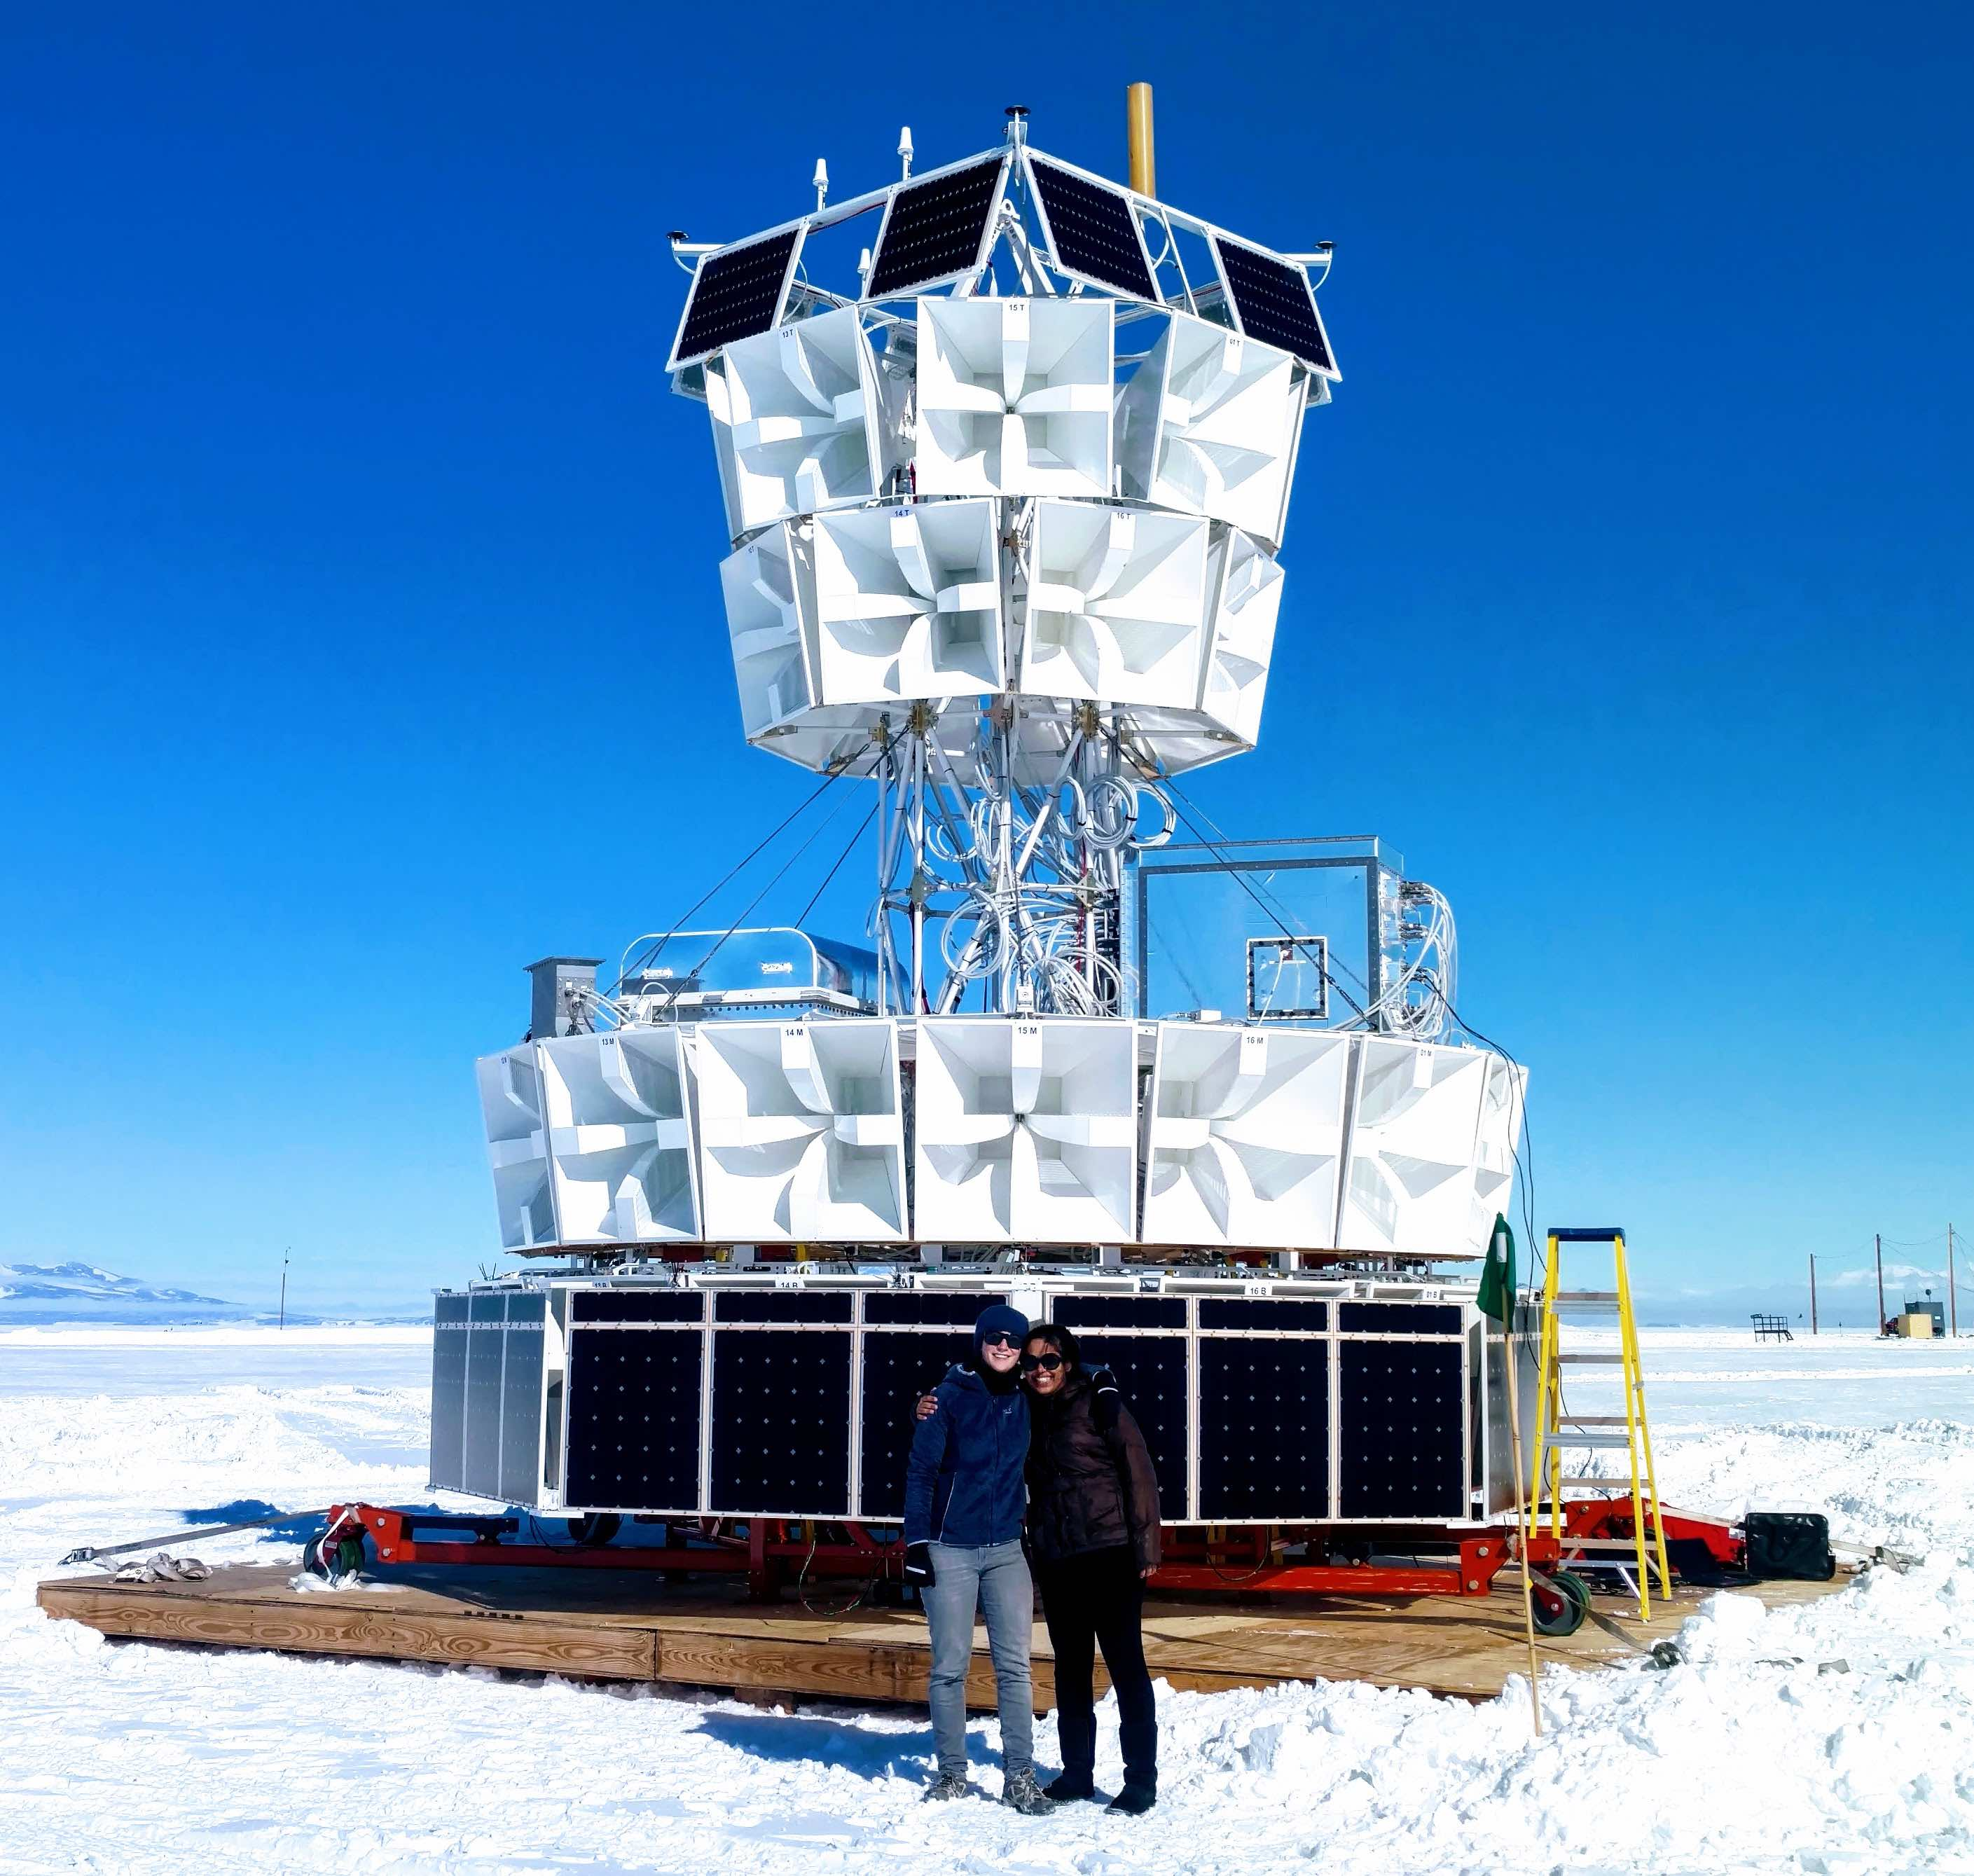
\includegraphics[width=1.0\textwidth]{figures/anita_thesis.jpg}
\caption{Linda Cremonesi and I during testing the GPS systems on ANITA-4 before its launch from near McMurdo Station, Antarctica. This shows the relative size of the instrument compared to humans. Picture credit: Steven Prohira.}
\label{my_anita}
\end{figure}

\begin{figure}
\centering
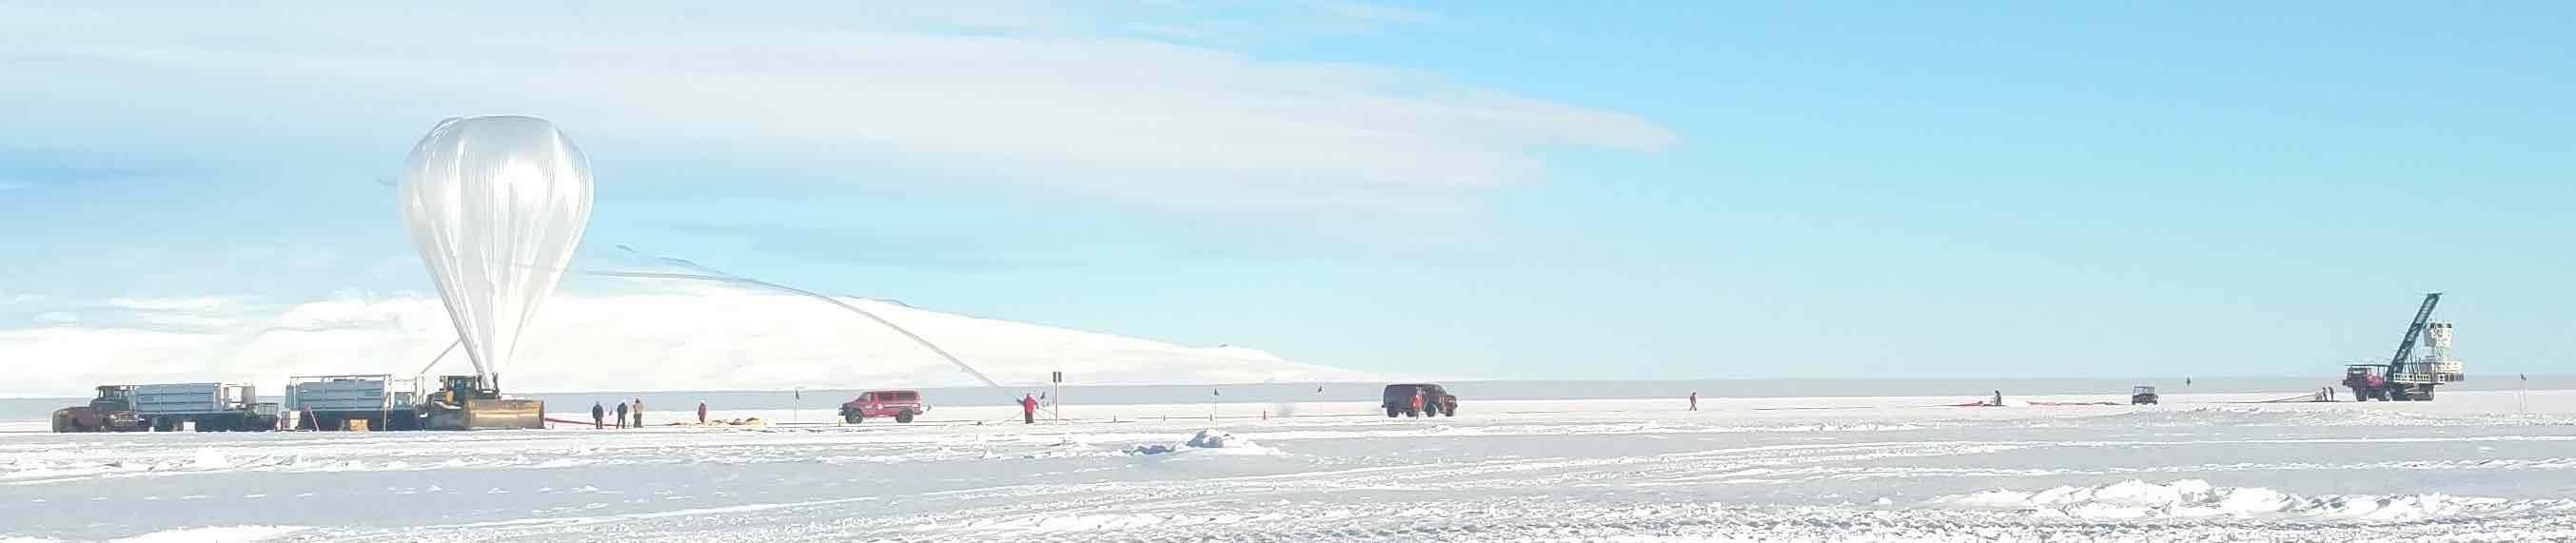
\includegraphics[width=1.0\textwidth]
{figures/launch_balloon.jpg}
\caption{Here NASA's balloon for the launch of ANITA-4 is being filled with Helium. When NASA takes the balloon out, one knows there will be a launch for real.}
\label{balloon_filled}
\end{figure}

\begin{figure}
\centering
\subfloat[ANITA-4 at launch]{
	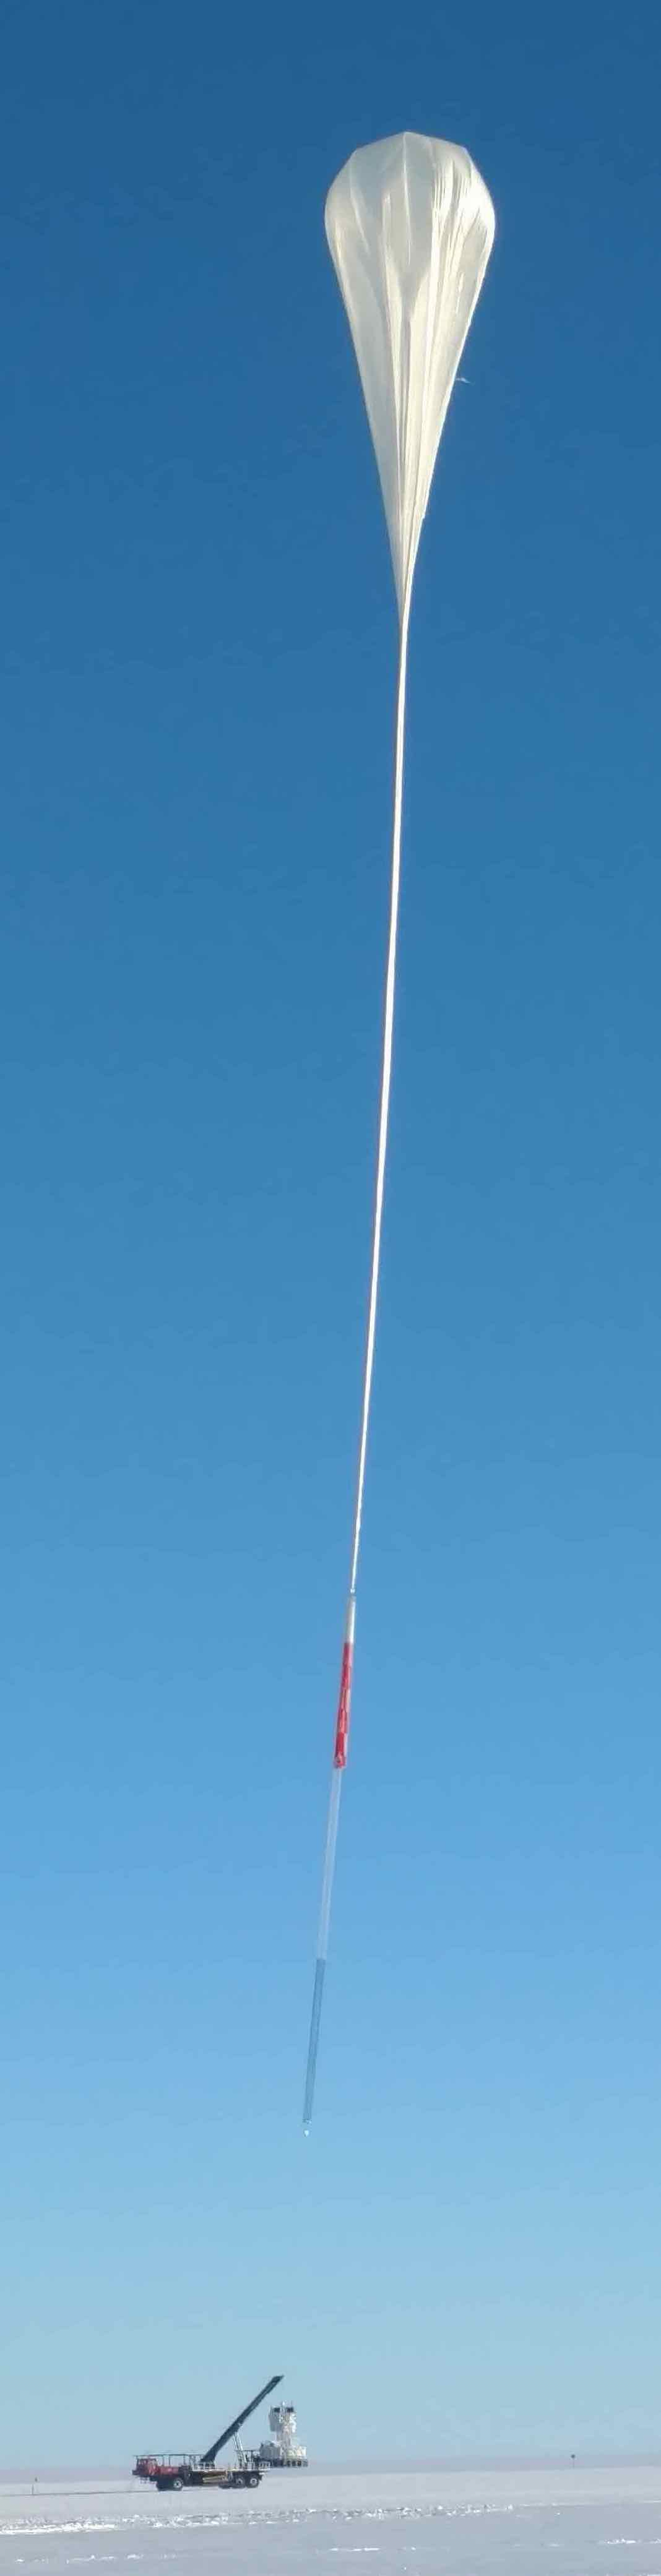
\includegraphics[width=0.24\textwidth]
	{figures/launch_thesis.jpg}
	\label{launch}
}
\subfloat[ANITA-4 at float altitude]{
	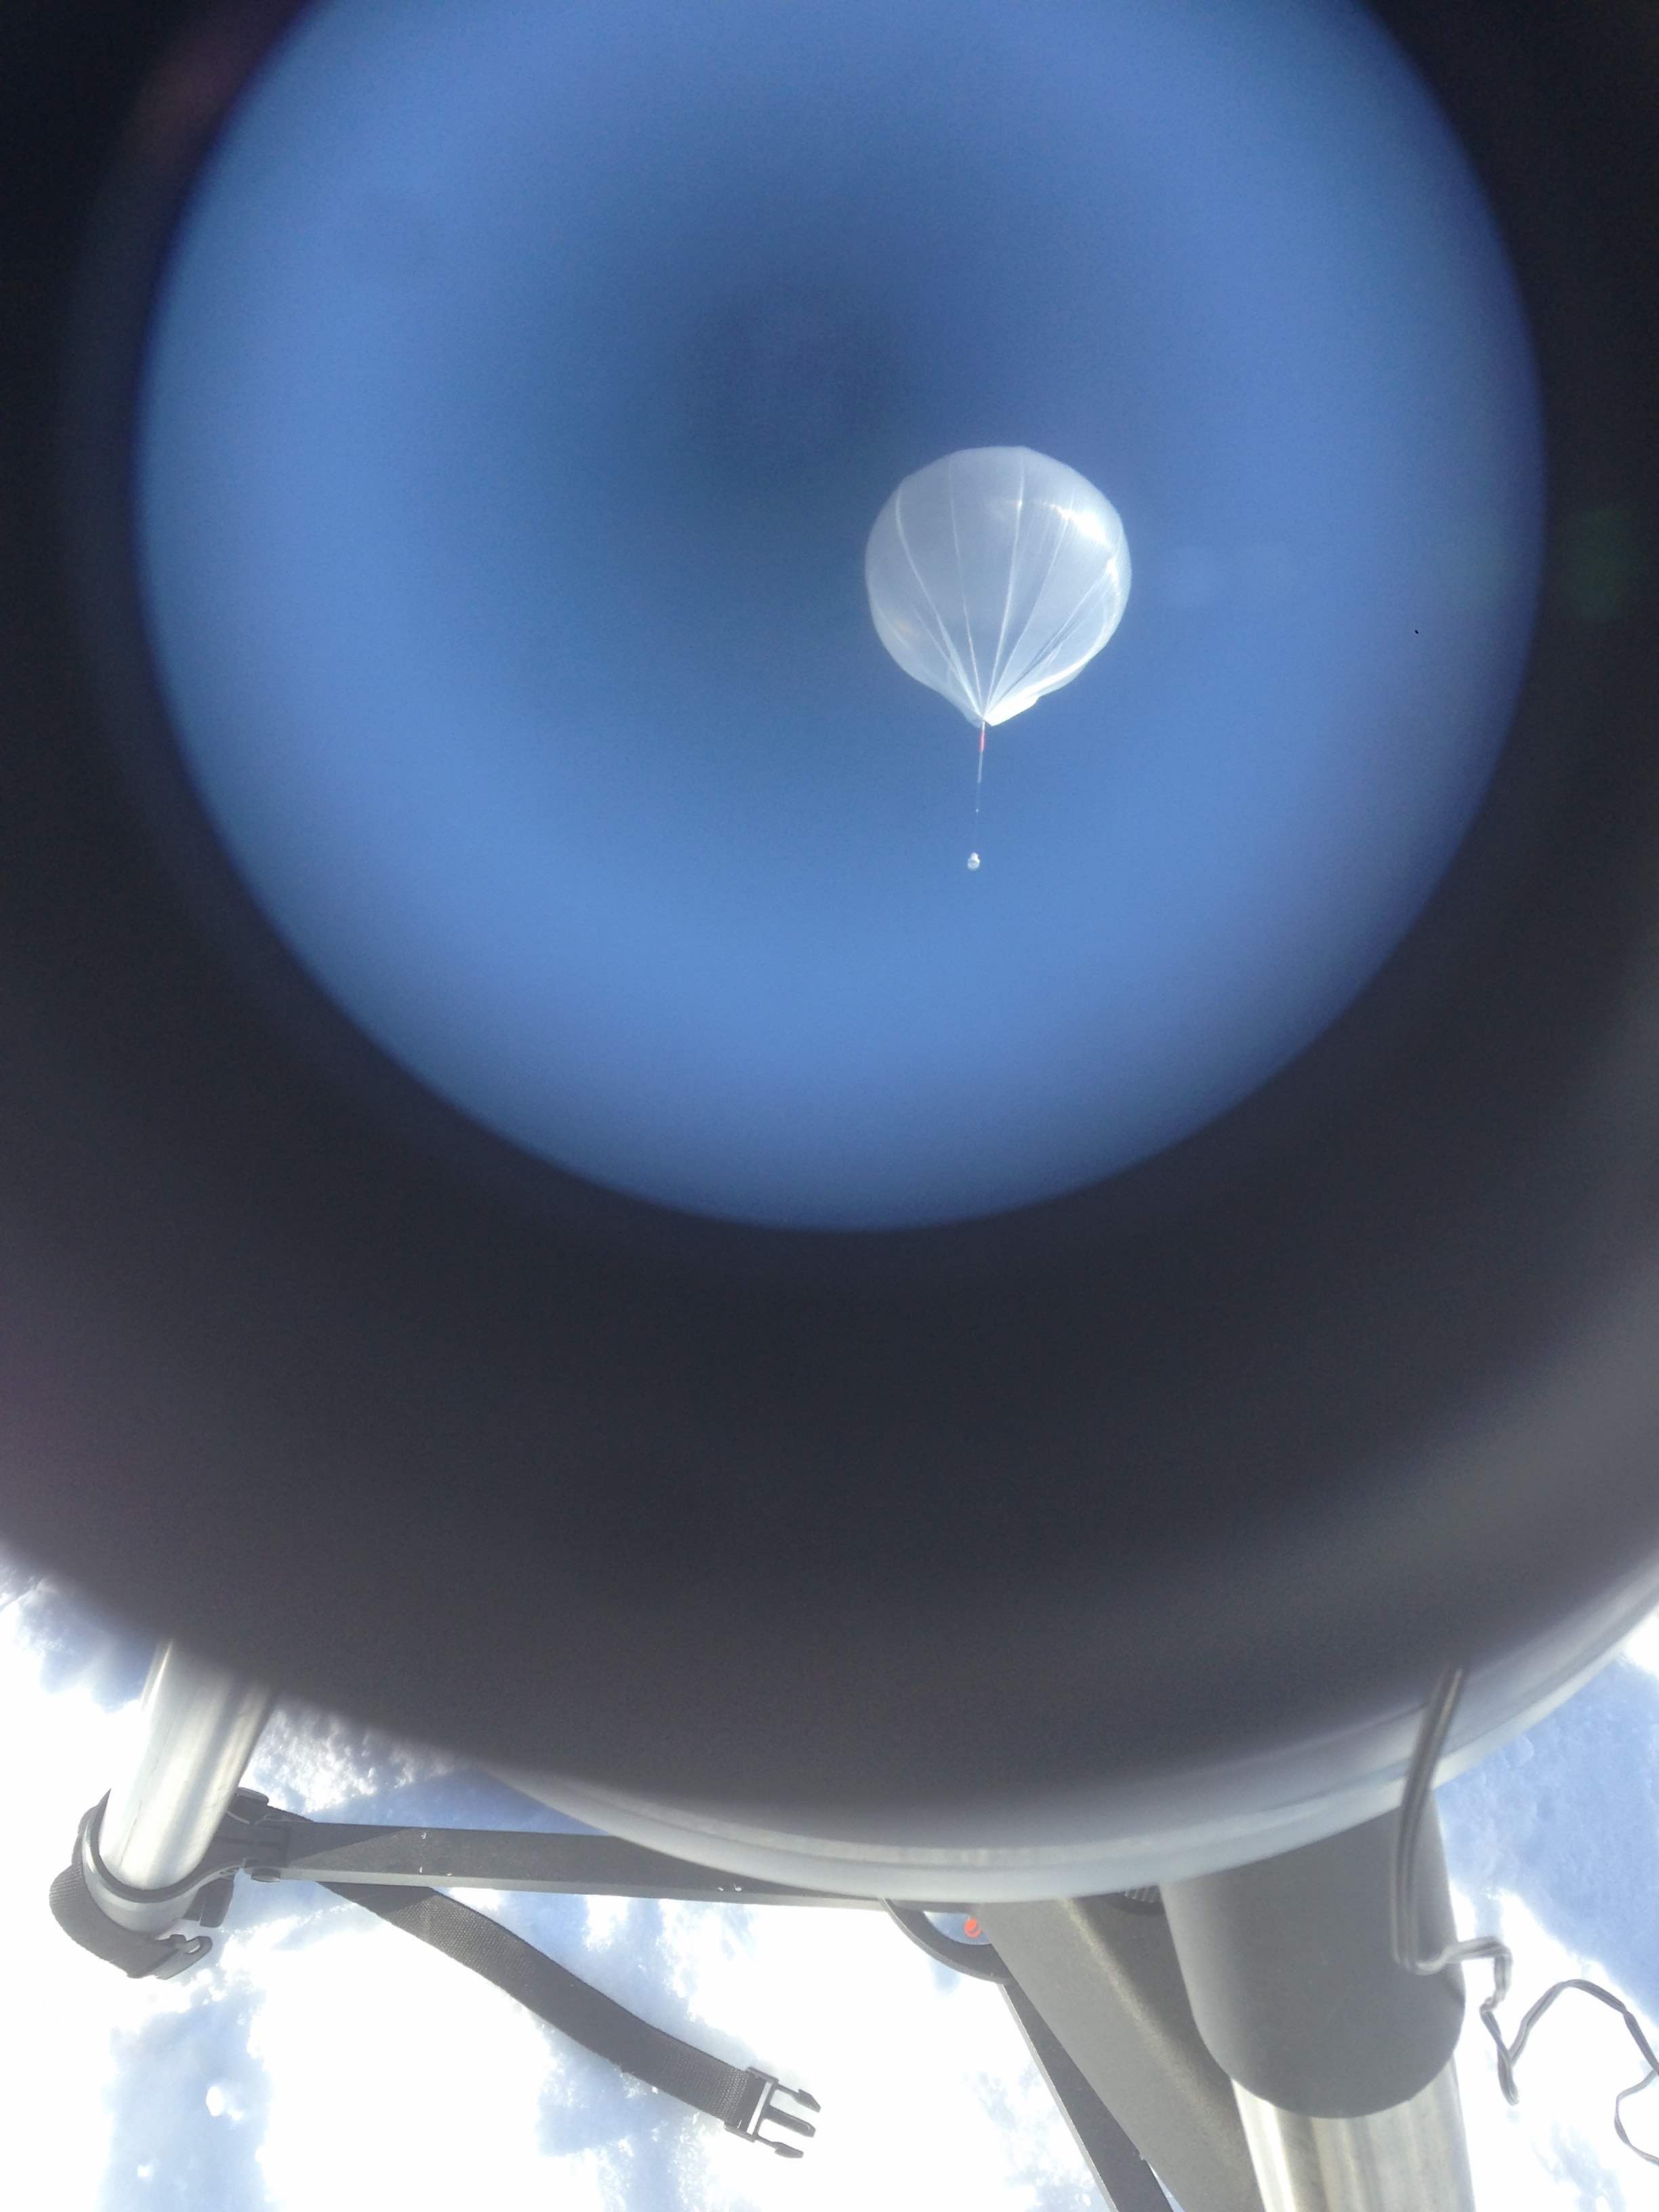
\includegraphics[width=0.7\textwidth]
	{figures/anita_float_big.jpg}
	\label{anita_float_big}
}
\caption{Left: The ANITA-4 payload attached to its balloon just before launch. Right: When ANITA gets close to its float altitude of about $40$ km, one cannot see it from the ground with the naked eye. This is ANITA-4 through a telescope. Telescope picture credit: Steven Prohira.}
\label{launch_float}
\end{figure}

\subsection{Flight path and payload weight}

The \gls{anita} neutrino observatory is a NASA long-duration balloon-borne payload.
After its launch from the NASA \gls{ldb} Facility near McMurdo Station,
the Summer polar vortex winds keep the ANITA payload flying in roughly circular loops above the continent of Antarctica. 
A lighter payload is able to reach higher altitudes where the polar vortex is spatially tighter. 
This leads to a more favorable flight path which, in turn, increases the chances of a longer flight and increased livetime. 
Most importantly, this 
keeps the payload from 
venturing out over the ocean and becoming unrecoverable. 

There are strict weight restrictions on a balloon payload. 
This is why
the \gls{anita} gondola is made of hollow aluminum tubes connected by joints. 
The aluminum beams can be seen in Figure~\ref{hanging}. 
A need for a light payload informed the design of the \gls{tuff} boards as detailed
in Section~\ref{tuff}. 
This helps to keep the payload weight under $5000\,\mbox{lb}$. 
The ANITA-4 payload weighed $4526\,\mbox{lb}$. 
For the first time, the \gls{anita}-4 payload was able to reach above $40\,\mbox{km}$ altitude for part of its flight. 
Furthermore, the ANITA-4 payload was able to maintain a more favorable flight path compared to the \gls{anita}-3 payload, resulting in a longer flight of 27 days compared to 22 days in \gls{anita}-3.

\begin{figure}
\centering
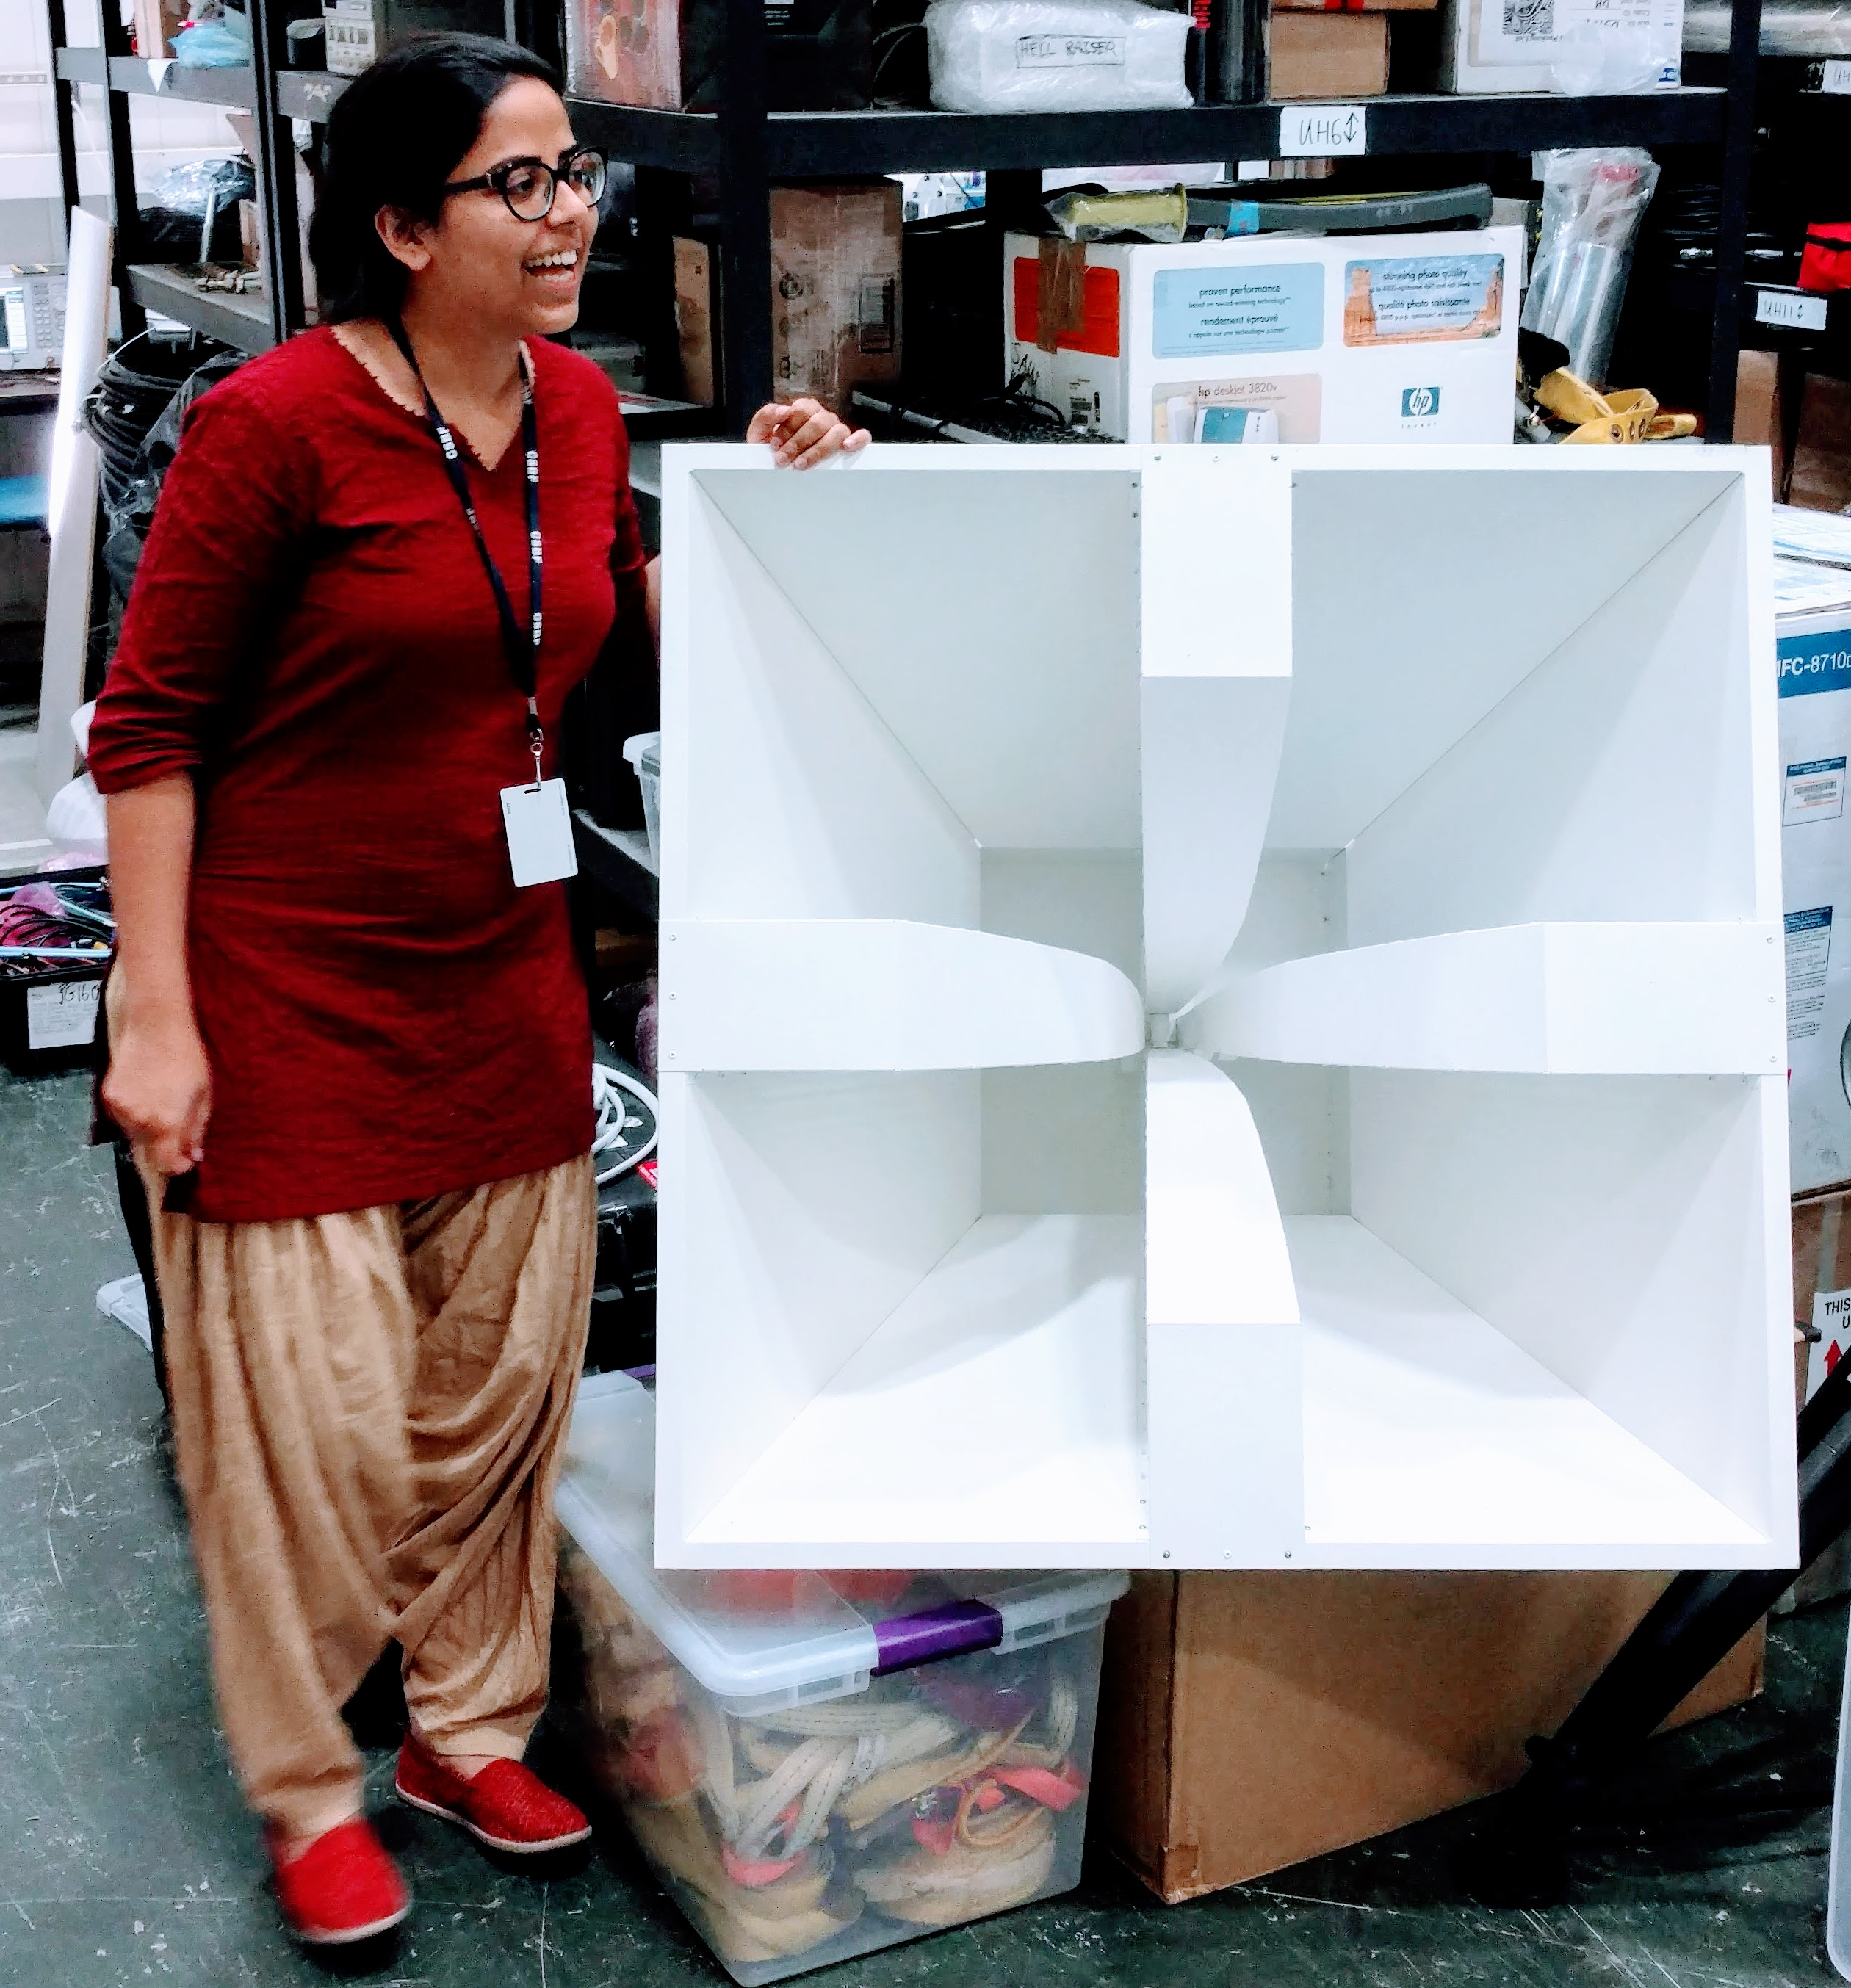
\includegraphics[width=1.0\textwidth]{figures/anita_antenna_me.jpg}
\caption{Here I am standing next to one of the ANITA horn antennas before the hang test of the ANITA-4 mission at Columbia Scientific Balloon Facility in Palestine, TX. Picture credit: Jacob Gordon.}
\label{antenna}
\end{figure}

\subsection{Radio antennas and Phi Sectors}

\gls{anita} looks for \gls{uhe} neutrinos with \gls{rf} antennas.
Figure~\ref{antenna} shows myself standing next to one of these antennas during the integration and testing of \gls{anita}-4 at the Columbia Scientific Balloon Facility in Palestine, TX in July of 2016. Custom-built by Seavey Engineering, they
are $0.8\,\mbox{m}$ long on a side, quad-ridged and horn-shaped.
The antennas are broadband and highly-directional. 
They have an on-axis gain of $\sim10\,\mbox{dB with respect to isotropic gain}$.
The $3\,\mbox{dB}$ point of these antennas is $\sim30^{\circ}$.


There are 48 antennas on the \gls{anita}-4 payload.
They are mounted on the ANITA gondola covering $360^{\circ}$ in azimuth. 
%Each antenna has two perpendicular feeds allowing detection of horizontally polarized and vertically polarized signals. 
%There have been 32, 40, 48, and 48 antennas on the \gls{anita}-1, 2, 3, and 4 flights, respectively.
The antennas are arranged in three aligned rings of 16 antennas, termed the top, middle, and bottom rings. 
The top ring consists of two staggered sub-rings each having eight antennas. 
%The antennas are mounted on the payload's gondola which is made of aluminum for its light-weight. 
The \gls{fwhm} beamwidth of the antennas is approximately $45^{\circ}$. 
The antennas in the top ring are evenly spaced by $45^{\circ}$ in azimuth. 
The two sub-rings in the top ring are offset by $22.5^{\circ}$ for uniform coverage.
The antennas in the middle ring are evenly spaced by $22.5^{\circ}$.
The antennas in the bottom ring are evenly spaced by $22.5^{\circ}$.
All the antennas are angled downward by $10^{\circ}$ to preferentially observe signals coming from the ice as opposed to from the sky. 
Each group of three antennas in a vertical column, taking one antenna from each ring, forms a phi sector, viewing a $22.5^{\circ}$ region in azimuth.

The antennas are dually-polarized with a feed each for \gls{hpol} and \gls{vpol} signal.
\gls{rf} signal through each channel goes through the 
\gls{ampa} unit before entering the Instrument Box. 
There is an \gls{ampa} unit connected directly to the \gls{hpol} and \gls{vpol} outputs of each antenna. 
The \gls{ampa} contains a $200 - 1200\,\mbox{MHz}$ bandpass filter, followed by an approximately $35\,\mathrm{dB}$ Low Noise Amplifier (LNA). The \gls{ampa} performs the first-stage amplification of the incoming \gls{rf} signal. I led a camp (John Russell christened it ``Campa") at the ANITA headquarters, University of Hawaii, in September of 2016, to finish assembling these \gls{ampa} units for the \gls{anita}-4 flight. I show one of the 100 that I worked on assembling in Figure~\ref{ampa}. These even involved a bit of careful soldering and using the heat gun!

\begin{figure}
\centering
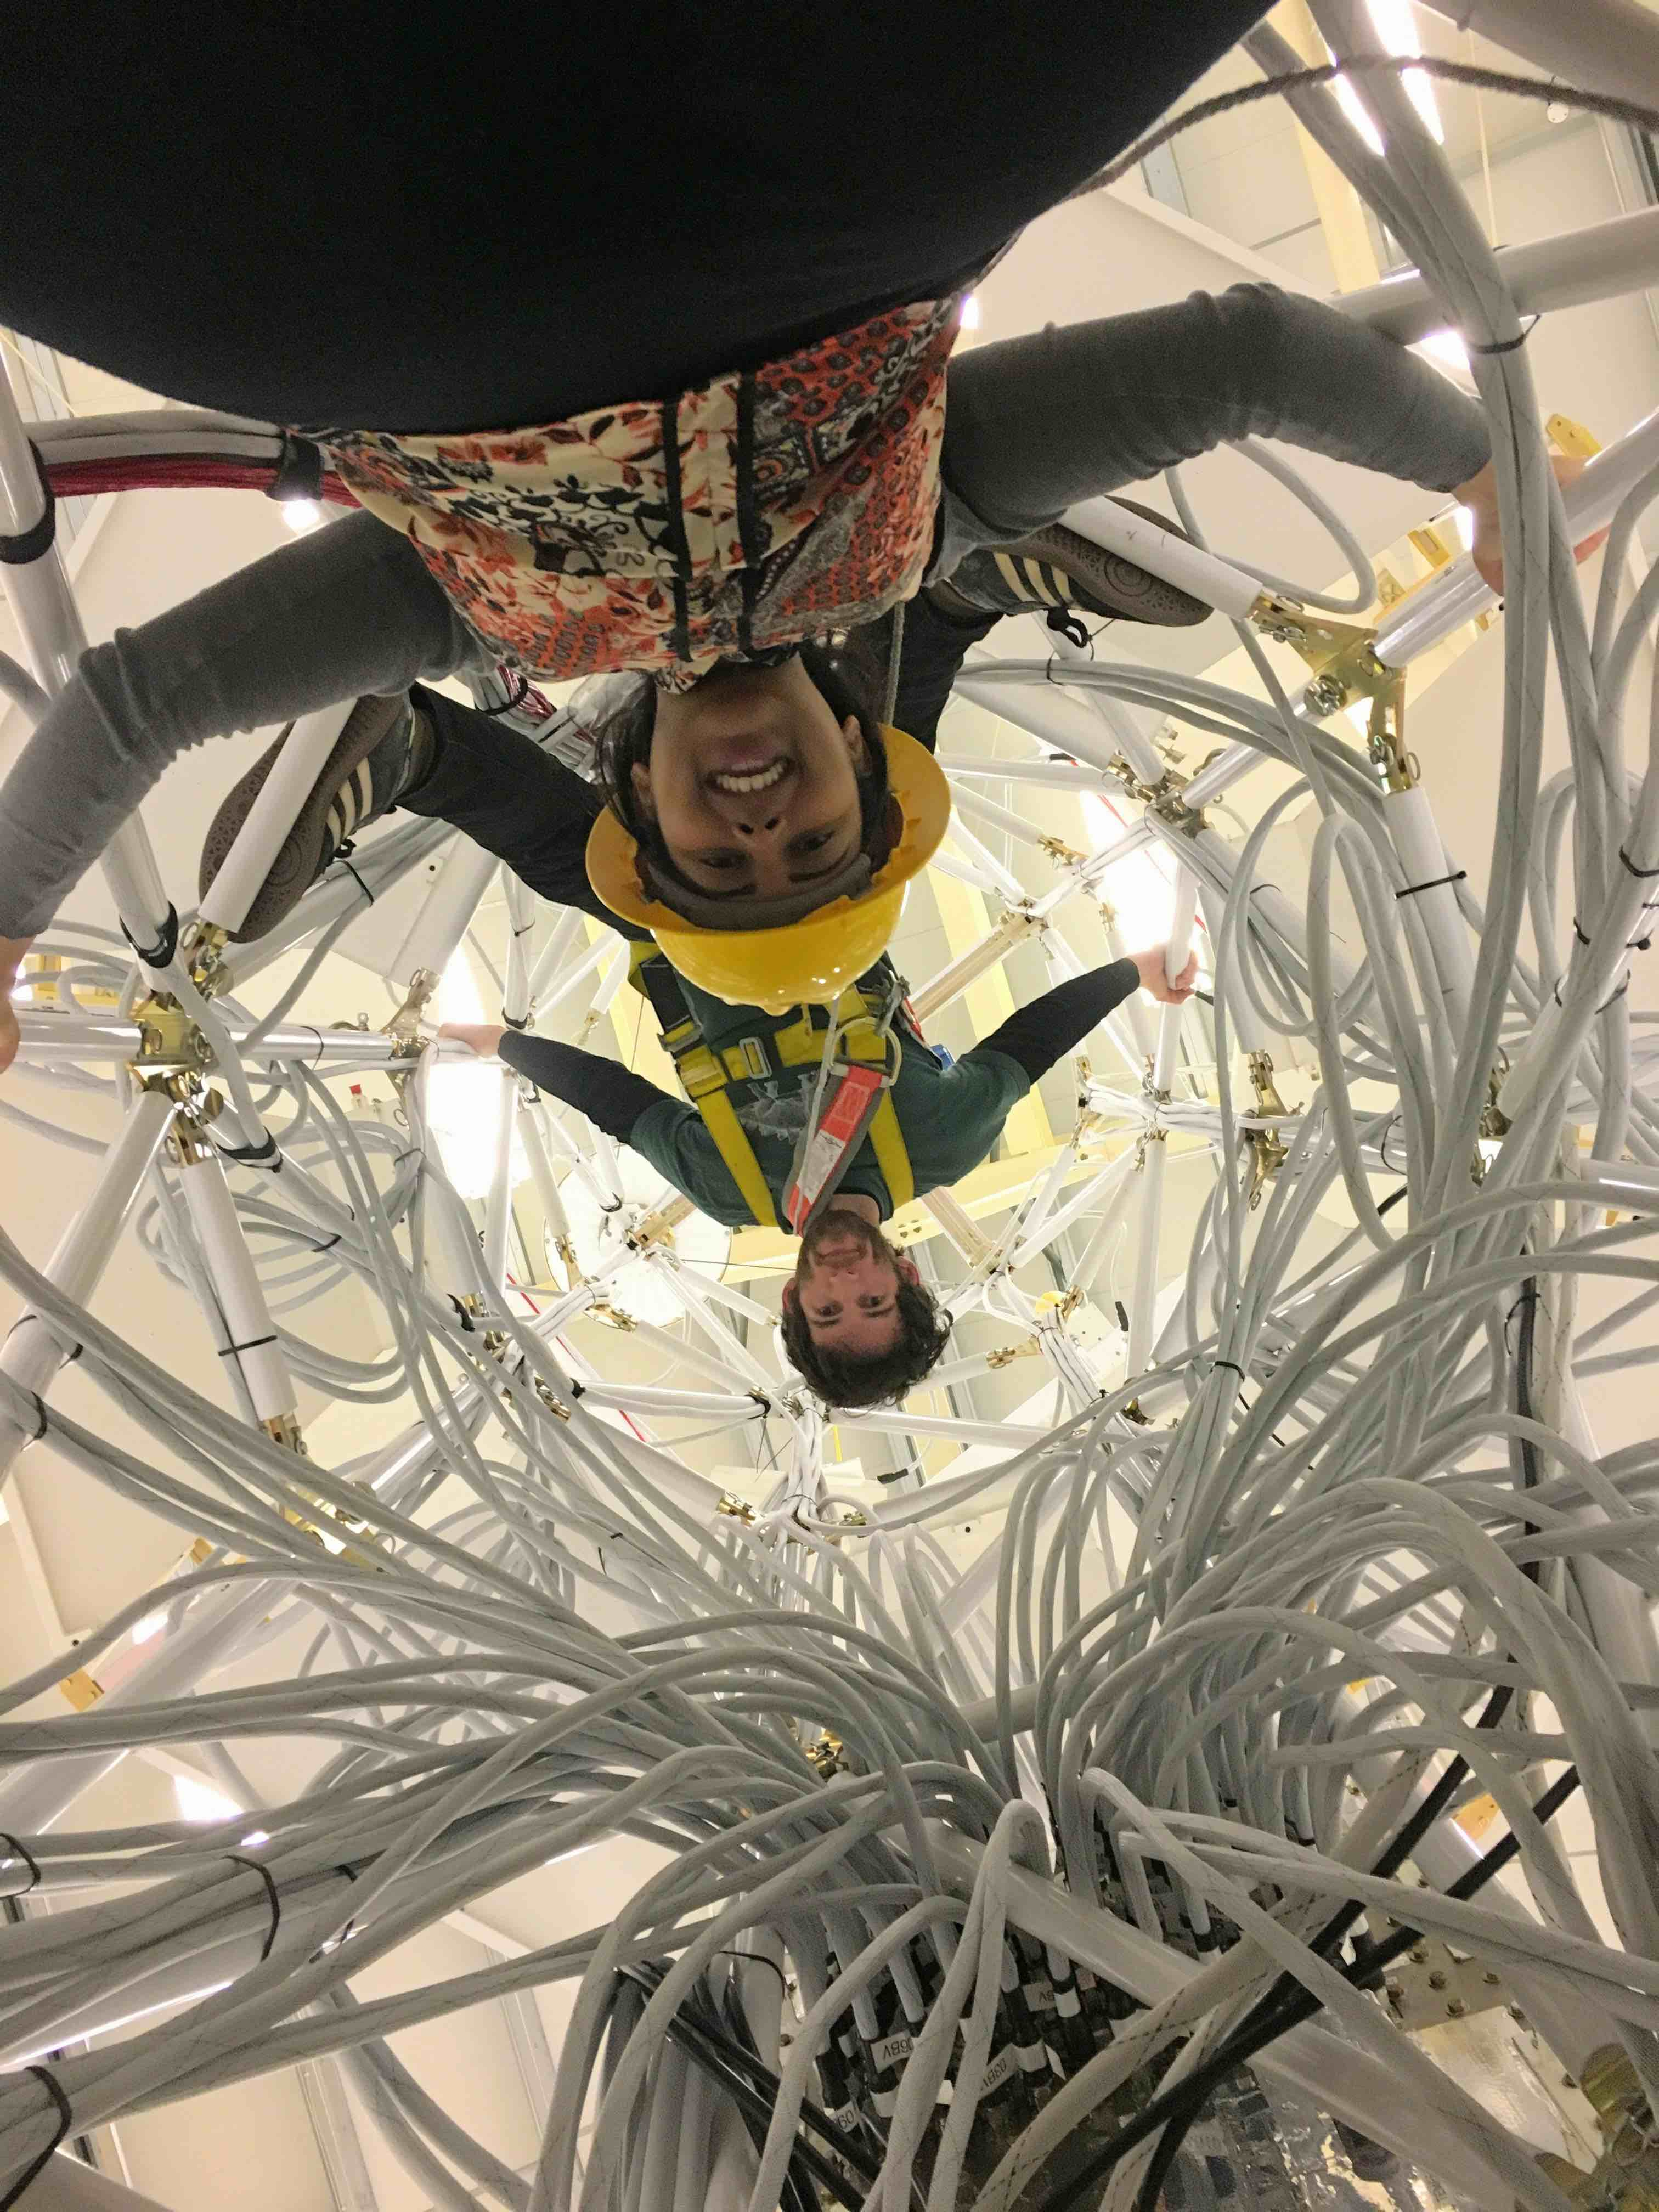
\includegraphics[width=0.52\textwidth]{figures/beams.jpg}
\caption{Andrew Ludwig and I working on integration and cabling of ANITA-4 at the NASA LDB facility near McMurdo Station, Antarctica. The aluminum beams that form the underlying structure of the payload can be seen here. Light aluminum beams help to abide by weight restrictions. Image credit: Nan Wang.}
\label{hanging}
\end{figure}

\begin{figure}
\centering
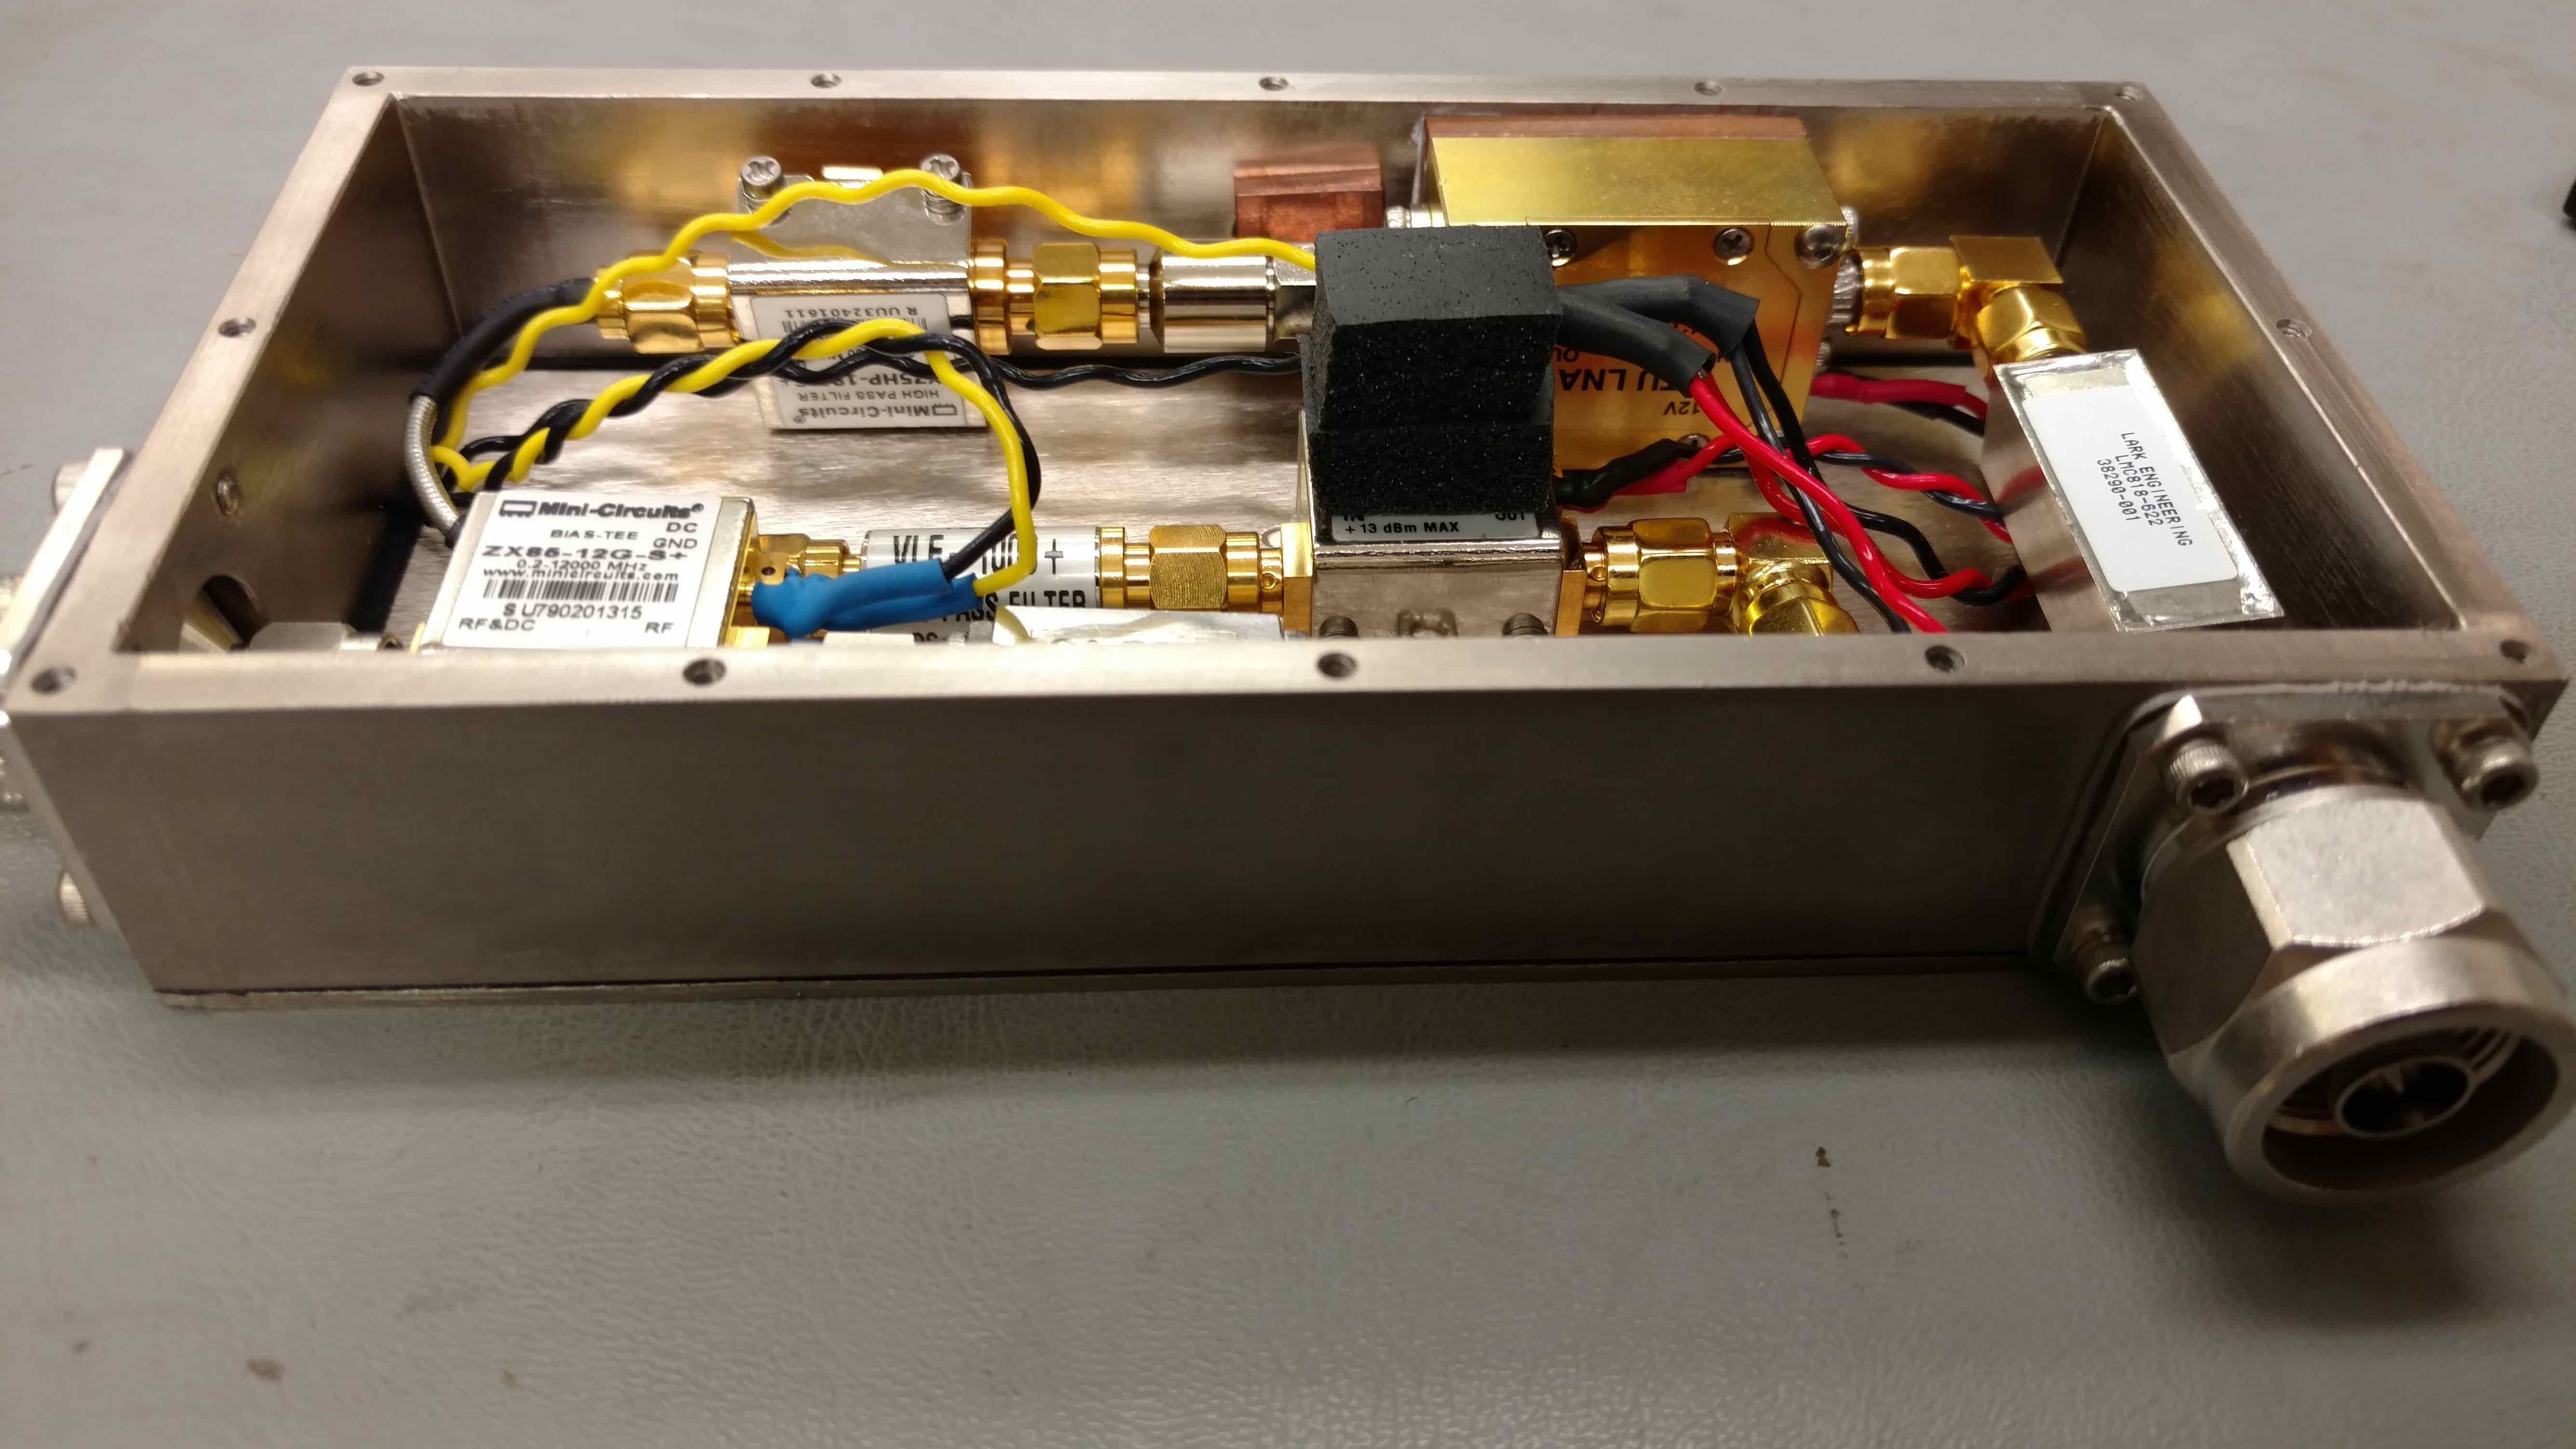
\includegraphics[width=1.0\textwidth]{figures/ampa.jpg}
\caption{Rare picture of the inside of an AMPA from ANITA-4.}
\label{ampa}
\end{figure}

\subsection{Instrument Box and Science Instrument Package}
\label{box_sip}

The Instrument Box of ANITA sits on the payload's deck. 
Most of the signal processing in \gls{anita} takes place inside the Instrument Box.  
Following the \gls{ampa} unit, the \gls{rf} signal travels through $12\,\mbox{m}$ of
LMR240 coaxial cable to the Instrument Box. 
Inside the Instrument Box, the signal first goes through second-stage amplification and notch filtering both performed by the \gls{tuff} boards in ANITA-4.
Then it passes through another set of bandpass filters before
being split into digitization and triggering paths. 
The triggering and digitization processes are detailed in~\cite{tuff}. 

The \gls{sip} also sits on the payload's deck. 
The SIP is powered and controlled by NASA.
It is used for flight control such as ballast release and flight termination. 
The SIP also provides a connection to the ANITA payload during flight through line-of-sight transmission, the Iridium satellite, and the Tracking and Data Satellite System (TDRSS). 
This allows us to monitor the payload continuously during the flight.
A small fraction of data (less than 1\%) is transferred from the payload through telemetry.
Commands to perform different functions, such as tuning a \gls{tuff} notch filter, 
%or altering a trigger threshold, 
can be sent to the payload in real time using the SIP connection. 

\subsection{Power}
\label{power}

There are unusual constraints on the total power budget of ANITA as it is a balloon payload. 
The ANITA-3 and ANITA-4 payloads operated on $\sim500\,\mathrm{W}$ and $\sim600\,\mathrm{W}$ respectively.
The payload is solar-powered by photovoltaic (PV) cells. 
One set of PV cells are on top of the gondola. 
These are managed by NASA and used to power the SIP. 
The other set is termed the ``drop-down PV array" and the PV cells in this set are arranged in eight 90-cell strings, laid out in an octagon around the bottom of
the payload. 
The drop-down PV array powers the Instrument Box. 
Before launch, they partially cover up the antennas in the bottom ring, as seen in Figure~\ref{anita}. 
After launch, the eight strings are remotely instructed to drop down by the SIP, which fires a servo to deploy them below the bottom ring of antennas. 

A charge controller distributes the output from the drop-down PV array to the payload as $24\,\mbox{V}$, using DC-DC converters 
to provide $12\,\mbox{V}$, $-12\,\mbox{V}$, $3.3\,\mbox{V}$ and $5\,\mbox{V}$ to various systems. 
The charge controller is also connected to a battery farm of $12\,\mbox{V}$ lead-acid batteries. 
Although there is daylight 24/7 in the Antarctic summer, the amount of power the PV array produces changes with the Sun's elevation during each 24 hour period. Thus, a battery farm is needed as backup. 
When the PV array is able to power the payload by itself, the charge controller charges the battery farm. 
This is in the Battery Box which is also placed on the deck. 

\subsection{GPS Systems and Heat dissipation} 
\label{gps_heat}

\gls{anita} data analysis relies on location and orientation information of the payload. 
\gls{anita} uses three GPS systems during flight: ADU5A, ADU5B and G12. 
These GPS antennas are located on top of the payload.
The ADU5 systems provide heading, pitch and roll information.
The G12 system updates absolute time on the flight computer through its Network Time Protocol (NTP) server. 
As backup to the GPS systems, there are four sun-sensor instruments, a magnetometer and accelerometer located on the deck. 

%\subsection{Heat dissipation}
At high altitudes of $35\,\mbox{km}$ and above, the primary method of heat loss is radiation. 
Thus, many parts of the payload are painted white to reflect sunlight and regulate temperature. 
Components producing large amounts of heat are connected to a teflon-coated, silver-tape-lined radiator plate on the Instrument Box.

\section{ANITA Signal Processing}

In this section we describe the signal processing chain for ANITA-4, and in particular
the steps that are relevant to understanding the role of the \gls{tuff} boards.
We will note when and where the ANITA-3 signal processing differed.
Note that much of the contents of this section is also covered in~\cite{tuff}. 
The \gls{rf} signal processing chain for ANITA-4 is illustrated in Figure~\ref{system}. 

\begin{figure}
\centering
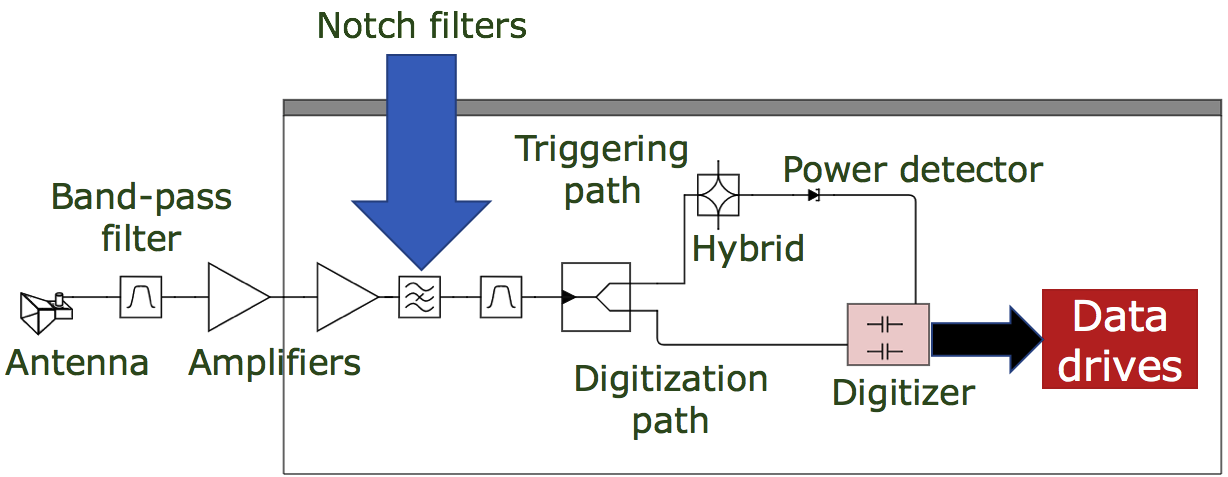
\includegraphics[width=1.0\textwidth]{figures/A4_simple_system.png}
\caption{Simplified form of the signal processing chain in ANITA-4. A more detailed diagram can be found in \cite{tuff}. The blue solid arrow shows where the TUFF notch filters are in the chain. More details on the TUFF boards and notch filters are presented later in this chapter.}
\label{system}
\end{figure}

\subsection{Triggering}
\label{trigger}

In the triggering path, the \gls{rf} signals from both the \gls{vpol} and \gls{hpol} channels of a single antenna 
are passed through a $90^{\circ}$ hybrid (hybrids were absent in ANITA-3). 
The outputs from the $90^{\circ}$ hybrid are the left- and right- circular polarized
(LCP and RCP) components of the combined \gls{vpol} and \gls{hpol} signals from an antenna. 
The hybrid outputs are input to the SURF (Sampling Unit for \gls{rf}) high-occupancy \gls{rf} Trigger (SHORT) unit before being passed to the SURF board. 
Each SHORT takes four channels as its input. 
In a SHORT
channel, the \gls{rf} signal passes through a tunnel diode and an amplifier. 
The output of the SHORT is
approximately proportional to the square of the voltages
of the input \gls{rf} signal integrated over approximately $5\,\mbox{ns}$.
It is a measure of the power of the incoming signal and is typically a negative voltage.
The SHORT output is routed to a SURF trigger input where 
it enters a discriminator that compares this negative voltage in Digital-to-Analog Converter (DAC) counts to the output
of a software-controlled DAC threshold on the SURF, henceforth referred to as the SURF DAC threshold. 
The SURF DAC threshold is expressed in arbitrary units of DAC counts corresponding to voltages. Lower thresholds 
correspond to higher voltages and therefore, higher power of the incoming signal. 
The SURF DAC threshold can be changed during flight. Thresholds for the \gls{anita}-3 and -4 flights are shown in Figure~\ref{thresholds_fig}. 
During the ANITA-3 flight, CW interference overwhelmed the digitization system, forcing us to impose
frequent and large changes in the SURF DAC thresholds. 
%A comparison of SURF DAC thresholds between ANITA-3 and ANITA-4 is presented in Figure~\ref{thresholds}.
Note that the lower overall threshold for ANITA-4 is primarily due to the modified triggering scheme, 
which requires more overall coincidences between channels. 
The increased stability of the ANITA-4 thresholds, due to the CW mitigation schemes presented later, is clearly apparent.

\begin{figure}
\centering
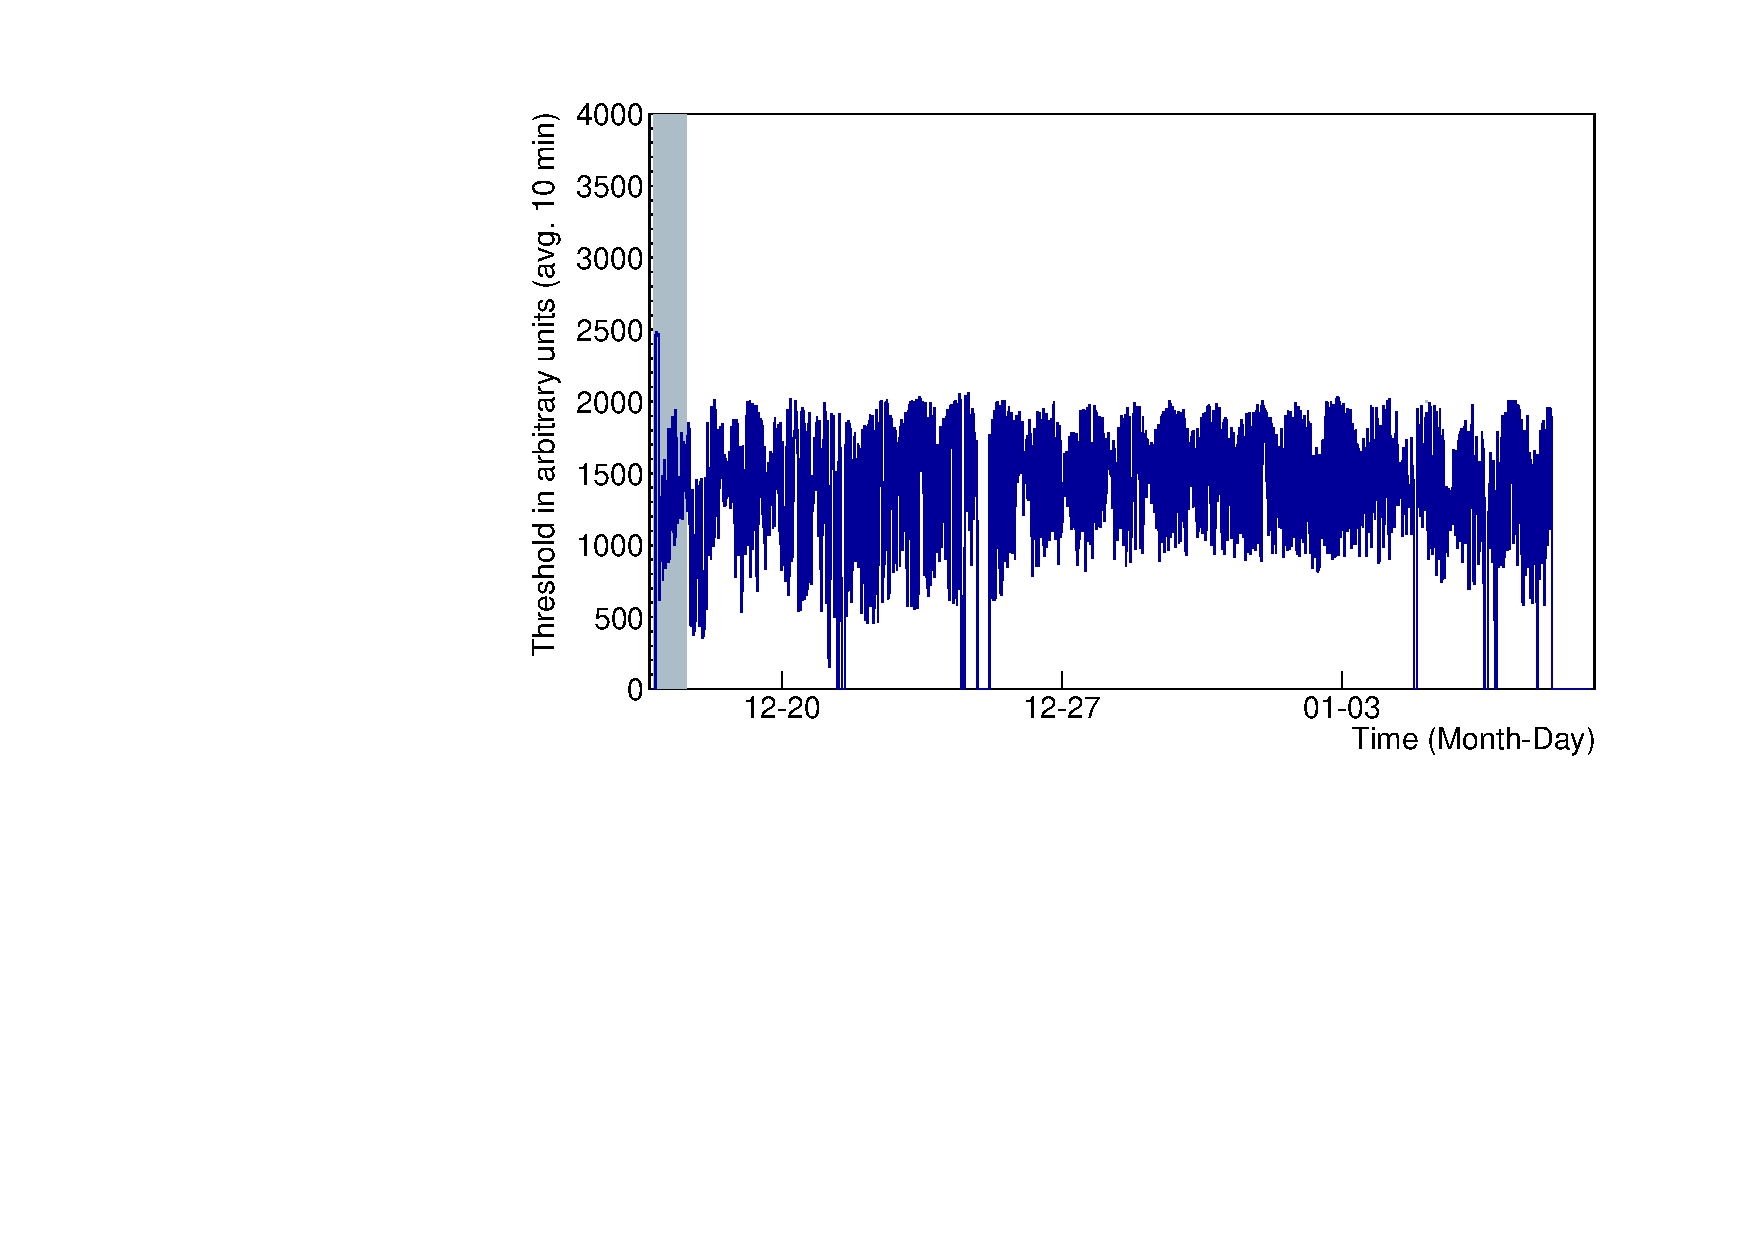
\includegraphics[width=1.0\textwidth]{figures/anita3_threshold_time20_2.pdf}
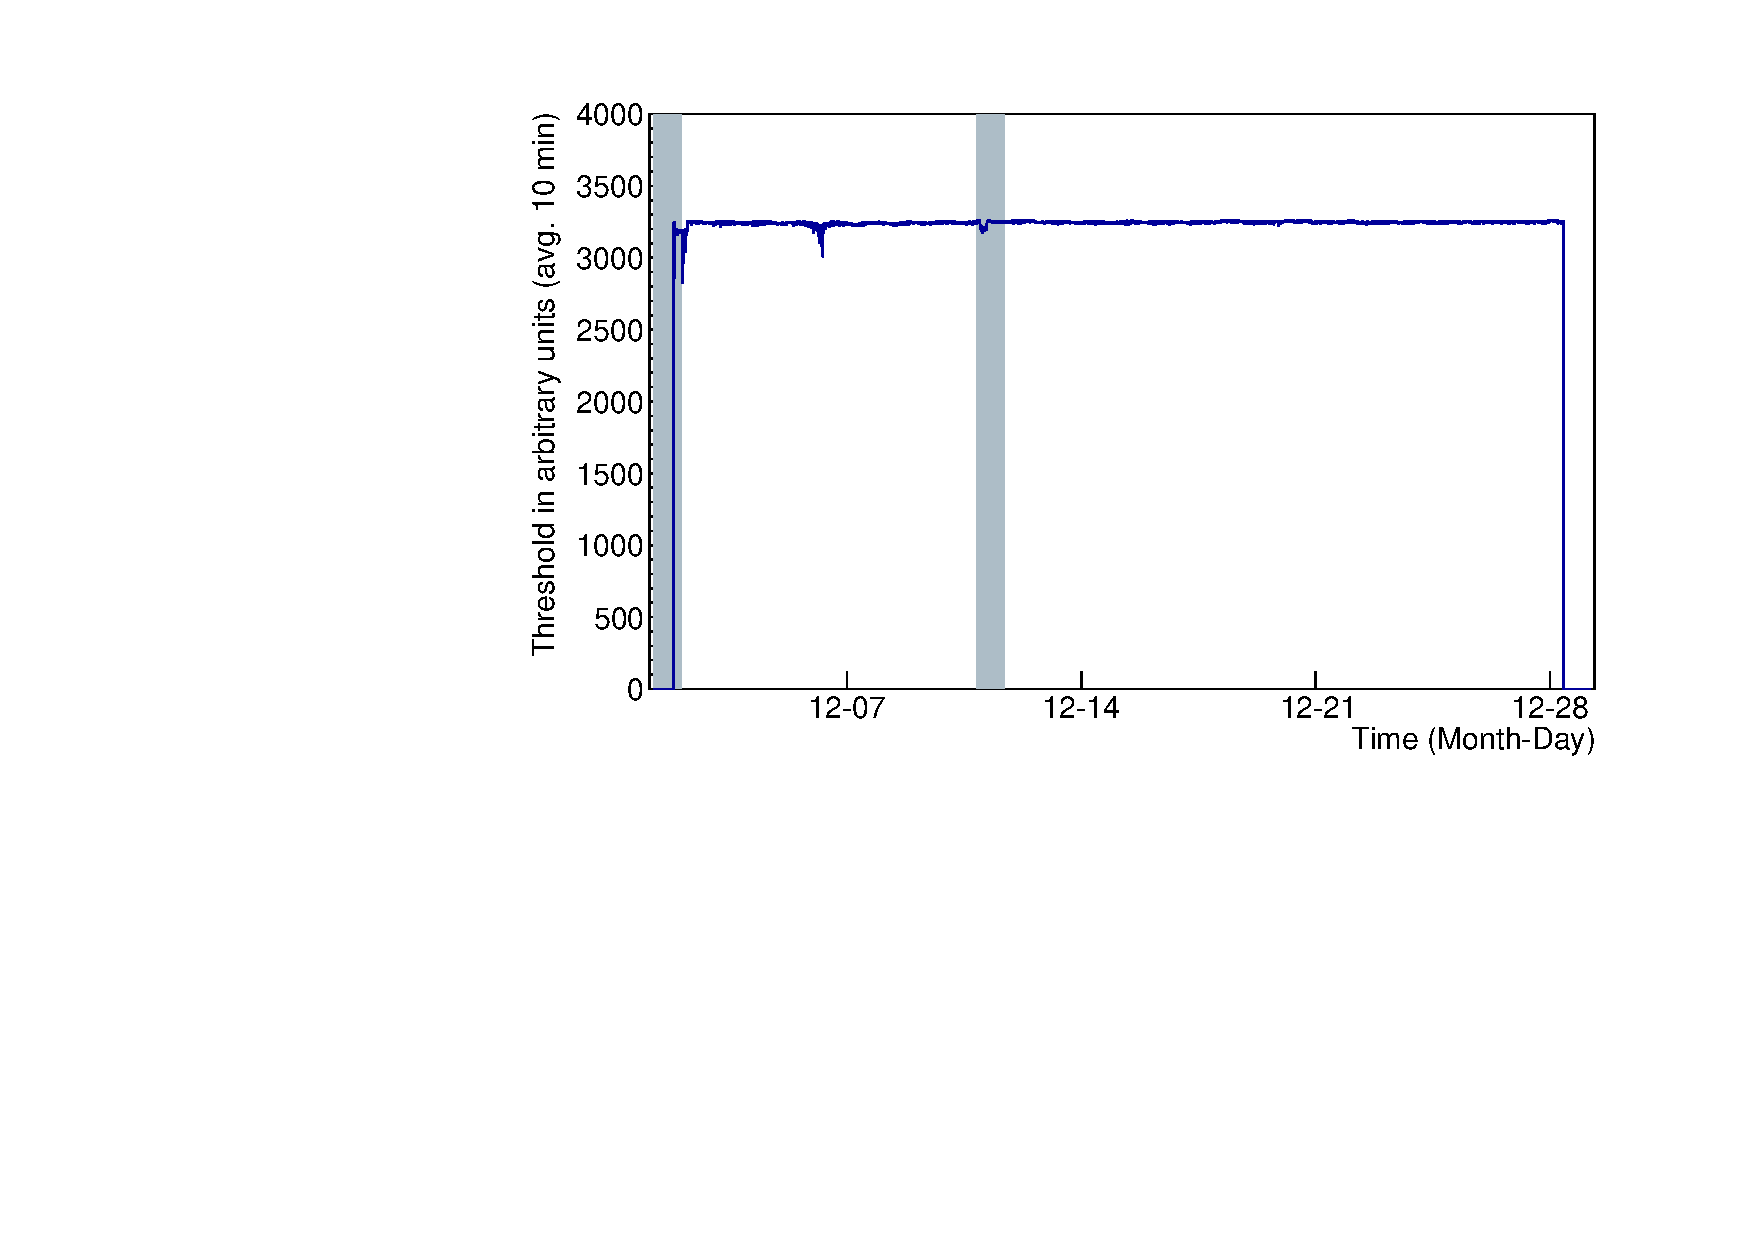
\includegraphics[width=1.0\textwidth]{figures/anita4_threshold_time_2.pdf}
\caption{Thresholds during the ANITA-3 (top) and ANITA-4 (bottom) flights.}
\label{thresholds_fig}
\end{figure}


\paragraph{Trigger logic:}
Due to power and bandwidth limitations, ANITA is not able to constantly record data. 
Digitization of data only occurs when the trigger conditions are satisfied.
The ANITA-4 trigger consists of three triggering levels: Level~1, Level~2 and Level~3. 
The trigger requirements at each of these three levels is described below.

\paragraph{Level~1 trigger:}

The Sampling Unit for \gls{rf} (SURF) board issues the Level~1 trigger.
To form a Level~1 trigger, the SHORT outputs of the LCP and RCP channels from the same antenna 
are required to exceed the SURF DAC threshold within $4\,\mbox{ns}$. This LCP/RCP coincidence requirement 
was added to the ANITA-4 trigger to mitigate anthropogenic and thermal backgrounds.
The signals of
interest are known to be linearly polarized, whereas satellite emission is often circularly polarized
and thermal noise is unpolarized. In the presence of a continuous source of CW signal such as satellites,
the LCP/RCP coincidence may still allow a combination of circularly polarized satellite noise and the circularly polarized component of
thermal noise to satisfy the Level~1 trigger requirement. Therefore, the LCP/RCP coincidence aids in
reducing triggers induced by satellites but does not completely mitigate their effect.

\paragraph{Level~2 trigger:} 

The SURF board issues the Level~2 trigger. 
A Level~1 trigger opens up a time window.
If there are two Level~1 triggers in the same phi sector within the allowable time window, then a Level~2 trigger is issued. 
The allowable time window depends on which antenna had the first Level~1 trigger. 
Time windows of
$16\,\mbox{ns}$, $12\,\mbox{ns}$ and $4\,\mbox{ns}$ in duration are
opened up when a Level~1 trigger is issued in the bottom, middle and top ring respectively.
These time windows were chosen to preferentially select signals coming up from the ice. 
The Level~2 trigger decisions are passed from the SURF boards to a dedicated triggering board called the Triggering Unit for \gls{rf} (TURF).
The Level~2 trigger timing in ANITA-4 differed from that used in ANITA-3 as changes were made to further restrict
the allowed timing of the antenna coincidences to 
better match timing expected from an incoming plane wave.

\paragraph{Level~3 trigger:}

The TURF board issues the Level~3 trigger.
A field programmable gate array (FPGA) on the TURF board monitors Level~2 triggers.
A Level~3 trigger is issued by the TURF board when there are Level~2 triggers in two adjacent phi sectors within $10\,\mbox{ns}$. 
When there is a Level~3 trigger, the TURF board instructs 
the SURF board to begin digitization.

\subsection{Digitization}

The digitization of the signal is performed by the SURF board. 
There are twelve SURF boards, each containing four custom-built Application Specific Integrated
Circuits called \gls{lab}. 

\paragraph{\gls{lab} chip and digitization deadtime:}
ANITA-4 uses the third generation
of \gls{lab} chips that are described by Varner \textit{et al}. \cite{labrador}. 
Each \gls{lab} chip has a 260-element switched capacitor array (SCA) for each of its 9 input channels, with one channel used for timing synchronization.
The \gls{rf} signal entering a SURF gets split and fed into four parallel \gls{lab} chips (forming four ``buffers" for digitization). 
The SCAs sample waveform data at the rate of $2.6\,\mbox{GSa/s}$. 
At any moment, the charge stored in an SCA is a $100\,\mbox{ns}$ record of the signal voltage. 
This $100\,\mbox{ns}$ snapshot of the incoming plane wave is known as an ``event."
When a Level~3 trigger occurs, a single \gls{lab} chip stops sampling and is ``held.'' It then digitizes
the stored data, which is then read out by the flight computer, taking approximately $5-10\,\mbox{ms}$.
If all four \gls{lab} chips are held, the trigger is ``dead'' and the accumulated time when the trigger is dead is recorded as
digitization deadtime by the TURF board. 

\paragraph{Masking:}

During ANITA-3, digitization deadtime due to high levels of anthropogenic noise was reduced
by excluding
certain phi sectors from participating in the Level~3 trigger. 
This is called phi-masking. 
Alternatively, specific channels (each antenna has two channels) were excluded from participating in the Level~1 trigger. 
This is called channel-masking.
Together these are referred to as masking.
Because of CW interference by military communications
satellites, over half of the payload had to be masked
during most of the ANITA-3 flight. 
This strongly motivated the creation of the \gls{tuff}
boards with tunable, switchable notch filters. 
%A comparison of masking between \gls{anita}-3 and \gls{anita}-4 is presented in Figure~\ref{phimasking}. 

\paragraph{Data storage:}
All \gls{anita} data is stored on-board with less than 1\% of it transmitted to the ground during flight by telemetry. This is why payload recovery is critical. 
The primary storage devices are two
HGST UltraStar He6 disks, each with $6\,\mathrm{TB}$ capacity. 
These two Helium
drives contain identical copies of the data for redundancy in case of a drive failure.
Additionally, there are six $1\,\mathrm{TB}$ Solid State Drives for secondary data storage. 

\section{Tunable Universal Filter Frontend}
\label{tuff}

For ANITA-4, we built and deployed 16 \gls{tuff} boards (not counting spares) with 
six channels each for the 96 total full-band \gls{rf} channels of ANITA. 
Figure~\ref{system} shows, for a single \gls{rf} channel in ANITA-4, where 
the \gls{tuff} boards are in the signal processing chain. Details on these boards, their function and performance, as well as a portion of the contents of this section, are presented in~\cite{tuff}. 
%However, most of the images that I include in this thesis are not already shown in the publication.

\subsection{The problem: modulated continuous wave interference} 

The principal challenge of the \gls{anita} experiment is to distinguish neutrino signals from \gls{rf} noise. 
The two main sources of noise are thermal radiation by the Antarctic ice and anthropogenic noise, much of which is modulated \gls{cw} interference. 

While Antarctica itself is relatively free of \gls{cw} transmissions, except for bases of human activity, transmissions from geosynchronous satellites are continuously in view.
The average \gls{fwhm} beamwidth of the \gls{anita} antennas is approximately $45^{\circ}$.
Although the \gls{anita} antennas are canted downward by $10^{\circ}$, the beam of the antennas extends to horizontal from the perspective of the payload and
above.  
The Antarctic science bases, the most prominent being McMurdo and South Pole Station, are more radio-loud than the rest of the continent, producing \gls{cw} interference, for example, in the $430-460\,\mbox{MHz}$ band. 

\begin{figure}
\centering
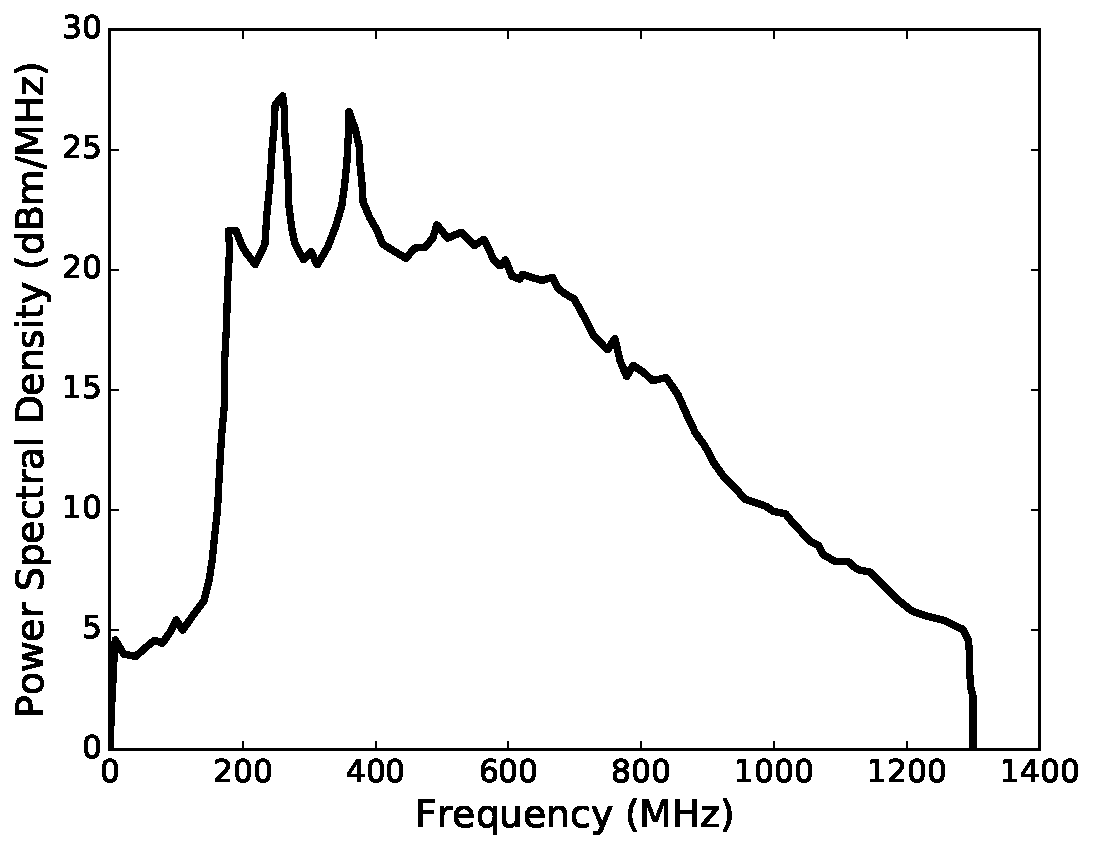
\includegraphics[width=1.0\textwidth]{figures/anita3spectra_wais_replot.pdf}
\caption{This averaged (over 2 mins) power spectrum shows the two CW peaks caused by military satellites that greatly reduced the instrument livetime (instrument livetime was only 31.6\%) of the ANITA-3 flight.}
\label{cw_peaks}
\end{figure}

\gls{cw} interference due to military satellites has affected all \gls{anita} flights.
\gls{anita}-1 (Dec. 2006 - Jan. 2007) and \gls{anita}-2 (Dec. 2008 - Jan. 2009) observed \gls{cw} interference primarily in the $240-270\,\mbox{MHz}$ band, peaking
at $260\,\mbox{MHz}$. This frequency range is predominantly used by the aging Fleet Satellite (FLTSAT) Communications System 
and the Ultra High Frequency Follow-On (UFO) System, both serving the 
United States Department of Defense since year 1978 and 1993 respectively.
In addition to \gls{cw} interference at $260\,\mbox{MHz}$, ANITA-III (Dec. 2014 - Jan. 2015) observed \gls{cw} interference at $375\,\mbox{MHz}$
which is thought to be due to
the newer Mobile User Objective System (MUOS) satellites that were launched during the period from Feb. 2012 - June 2016 \cite{milsat}.
The \gls{cw} signals generate events with excess power in left circular polarization (shown for the first time in Stafford's thesis~\cite{samStaffordThesis}) above the horizon, in approximately stationary positions.

The \gls{anita}-3 experiment was most affected by \gls{cw} interference due to military satellites. The first and second peaks in the power spectrum shown in Figure~\ref{cw_peaks} were present during all and about half, respectively, of the \gls{anita}-3 flight.
Due to the design
of the \gls{anita}-1 and \gls{anita}-2 trigger, which required coincidences among different frequency bands, the \gls{cw} interference did not overwhelm
the acquisition system. 
However, \gls{anita}-3 was redesigned for improved sensitivity and based its trigger decisions on full-bandwidth ($200 - 1200\,\mbox{MHz}$) signals. 
The modulation present in the \gls{cw} interference produced trigger rates far in excess of the digitization system's readout capabilities ($\sim50\,\mbox{Hz}$) for thresholds comparable to those used in previous flights. 
Thus, the \gls{anita}-3 experiment was susceptible to digitization deadtime throughout the flight. 

The lesson learned from the \gls{anita}-3 flight was
that a new method of mitigation of \gls{cw} signal was critical for the \gls{anita}-4 flight. 
Before \gls{anita}-4, the available methods to reduce digitization deadtime were masking
and decreasing thresholds when in the presence of higher levels of noise. 
A decrease in thresholds corresponds to higher power of the incoming signal. 
Masking and decreasing thresholds
come at the cost of instrument livetime~\cite{tuff} and sensitivity to neutrinos, respectively. 
%Both of these methods come at a high price.
For about 90\% of the time during the \gls{anita}-3 flight,
masking was used 
%during noisy periods 
to veto triggers from
over 
half of the payload field-of-view to keep the
trigger rate at or below $50\,\mbox{Hz}$. 
This significantly lowered the total instrument livetime. 
%Decreasing thresholds led to reduction of sensitivity to neutrinos during noisy periods. 
For \gls{anita}-4, the \gls{tuff} boards were built with
tunable notch filters to restore triggering efficiencies 
in the presence of CW interference. 
Additionally, the $90^{\circ}$ hybrids, previously deployed in \gls{anita}-1 as described in our design paper \cite{instrPaper}, were added to the \gls{anita}-4 trigger system by requiring a coincidence between left- and right- circularly polarized signals.
 
\begin{figure}
\centering
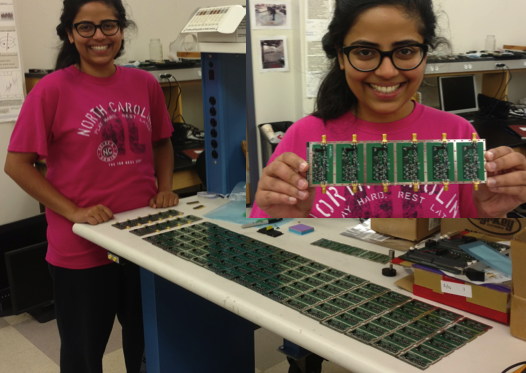
\includegraphics[width=1.0\textwidth]{figures/tuff_construction.png}
\caption{During the construction of the TUFF boards at OSU (May - July of 2016). The picture of myself holding one of the boards gives an idea for their size and shape. Clearly, building these boards made me very happy.}
\label{tuff_construction}
\end{figure}

\subsection{Design and construction}

In April of 2016, NASA gave the \gls{anita} collaboration the go ahead to attempt a launch of the \gls{anita}-4 mission at the end of that same year. From May - July of 2016, I worked on constructing and testing the \gls{tuff} boards. Constructing them involved soldering several thousand parts on to the boards. This was done by a small team at OSU, including myself, Jacob Gordon and Michael Kovacevich. Patrick Allison designed the boards and supervised our work. Testing of the boards was done in different stages and involved frequent measurement of the \gls{tuff} response using the network analyzer, making measurements of the board's current, capacitance, etc. with the multimeter, and performing experiments using the thermal and vacuum chambers. Figure~\ref{tuff_construction} shows myself holding a \gls{tuff} board and standing next to a freshly soldered batch of \gls{tuff} boards.

\begin{figure}
\centering
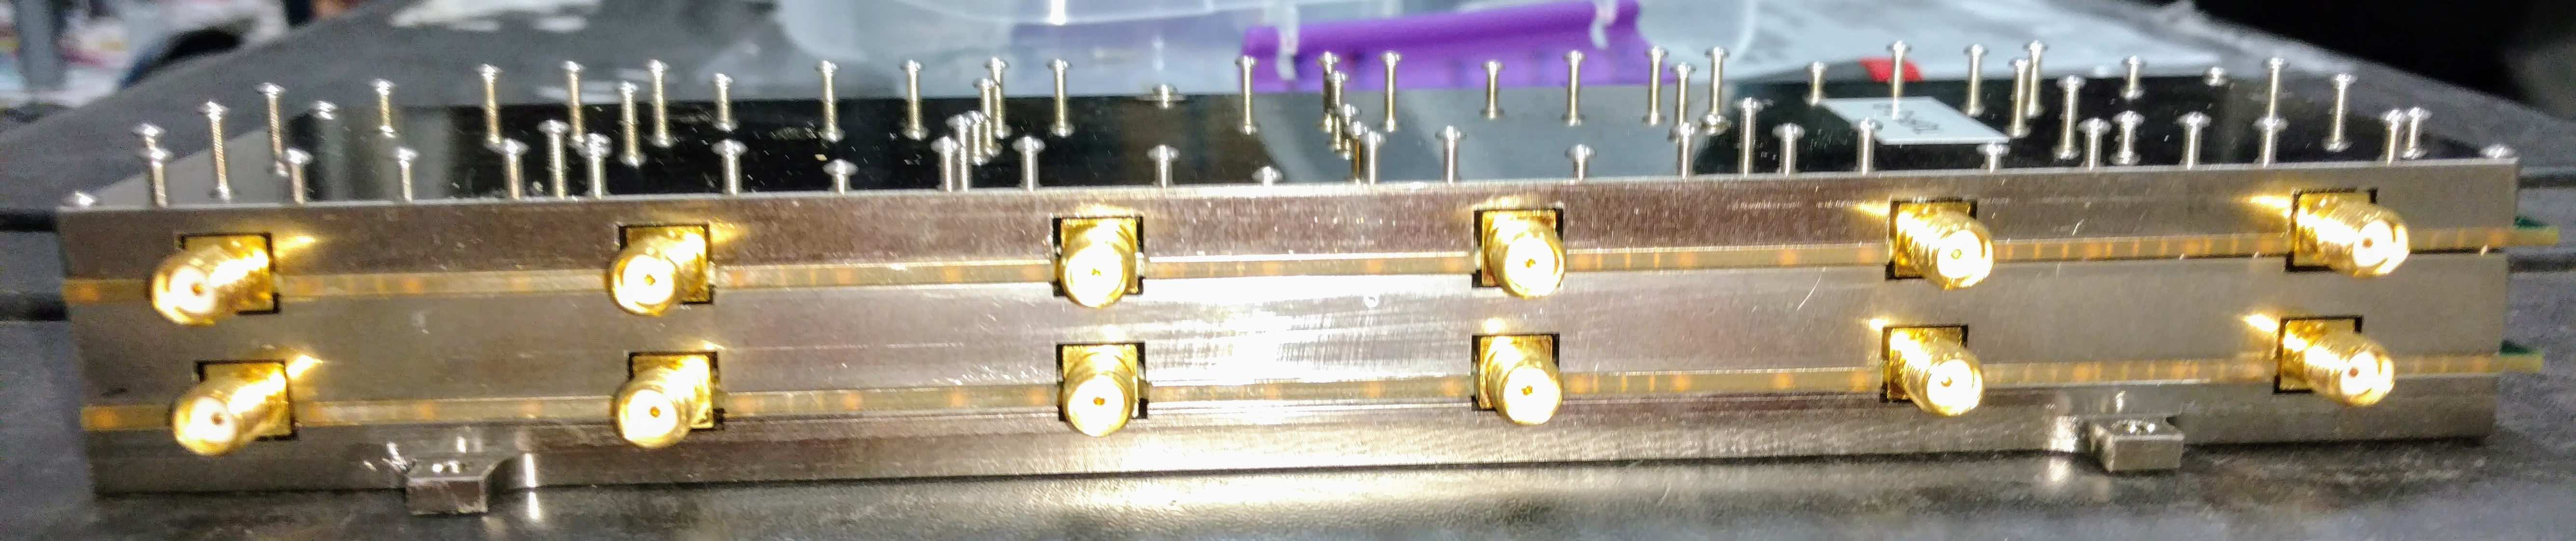
\includegraphics[width=1.0\textwidth]{figures/tuff_case_screws.jpg}
\caption{Pairs of TUFF boards were enclosed within aluminum cases with RF padding on the inside. The enclosures were held shut with the help of the screws shown here. Even a slight problem with the case design could make it very difficult to put the screws in or take them out. In fact, these screws became the bane of our existence during integration and testing of ANITA-4, and demonstrated how important it was to get the design of the cases right. Thanks to Christian Miki for designing the case.}
\label{case_screws}
\end{figure}

The design of the \gls{tuff} board was affected by the low power budget of \gls{anita} as well as the weight and size restrictions of a balloon mission, as described in Section~\ref{payload}. 
The \gls{tuff} boards needed to be low-power, compact and light. %Figure~\ref{tuff_channel} shows a single \gls{tuff} channel next to a quarter USD coin for size comparison. 
A single channel is about twice the size of a quarter dollar coin. 
Each printed circuit board has four layers of copper with an FR-4 dielectric material. 
%This is a composite made of woven fiberglass cloth with an epoxy resin binder that is flame resistant.
The \gls{tuff} boards operate on $3.3\,\mathrm{V}$ and $4.7\,\mathrm{V}$ power sources 
provided by
a MIC5504 from Microchip Technologies Inc. and a ADM7171 from Analog Devices Inc. Both
voltage regulators draw from a $5\,\mathrm{V}$ source 
supplied by the DC/DC unit in the ANITA
Instrument Box. 
A single \gls{tuff} channel consumes only $330\,\mathrm{mW}$ of power. 
The total power consumed by the ANITA payload is approximately $800\,\mathrm{W}$. 

Two \gls{tuff} boards were assembled into a final 
12-channel aluminum housing as shown in Figure~\ref{case_screws}. This provides heat-sinking, structural support, and \gls{rf} isolation. 
Two of these 12-channel modules were placed inside an 
\gls{irfcm} inside the Instrument Box of ANITA. Figure~\ref{irfcm} shows the inside of an IRFCM. Each \gls{tuff} channel has four main components which are described in the following subsections. 

\begin{figure}
\centering
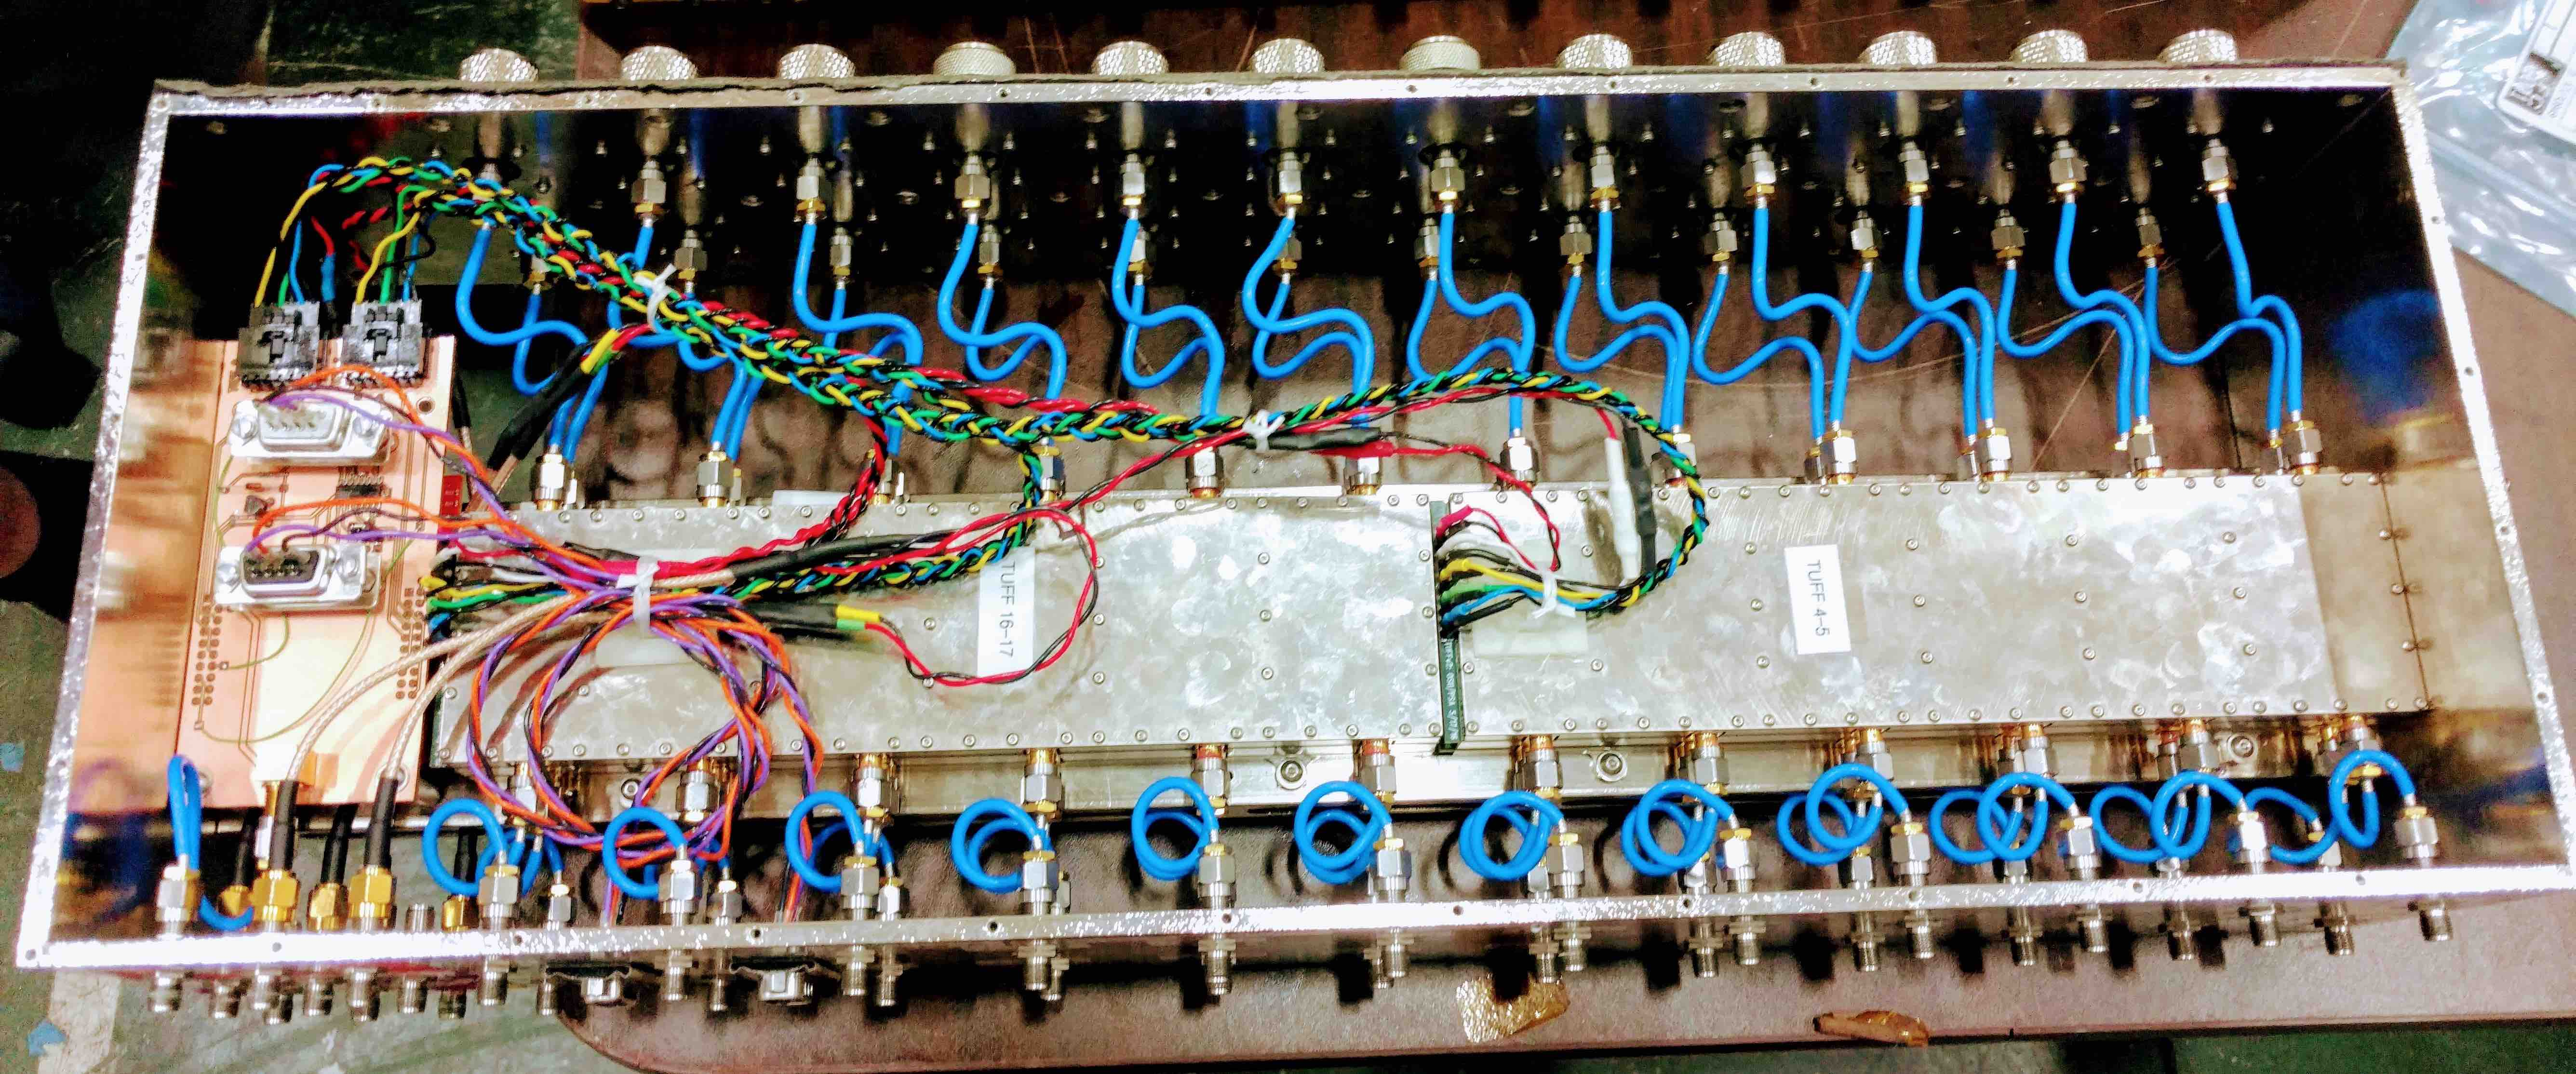
\includegraphics[width=1.0\textwidth]{figures/irfcm_thesis.jpg}
\caption{Rare picture of the inside of an Internal Radio Frequency Conditioning Module (IRFCM) holding two TUFF modules and a TUFF master. There are four total IRFCMs.}
\label{irfcm}
\end{figure}

\subsection{Amplifiers and bias tee} 

There are two amplifiers connected in series that together 
produce second-stage \gls{rf} power amplification of approximately $45\,\mathrm{dB}$. 
%The gain of a \gls{tuff} channel, as measured in the lab, is shown in Figure~\ref{s21}. 
AMP~1 is a BGA2851 by NXP Semiconductors and AMP~2 is an ADL5545 by Analog Devices. 
There is an attenuator producing $1\,\mathrm{dB}$ of 
attenuation to the \gls{rf} signal as it leaves
AMP~1 and before it enters AMP~2.
The BGA2851 provides a gain of $24.8\,\mathrm{dB}$ at $950\,\mbox{MHz}$. 
It has a noise figure~of $3.2\,\mathrm{dB}$ at $950\,\mbox{MHz}$. 
It consumes $7\,\mathrm{mA}$ of current at a supply voltage of $5\,\mathrm{V}$, 
or $35\,\mathrm{mW}$ of power.
The ADL5545 provides a gain of $24.1\,\mathrm{dB}$ with broadband operation from $30-6000\,\mbox{MHz}$.
Out-of-band power at frequencies above $2\,\mbox{GHz}$ is suppressed by a filter on each \gls{tuff} channel. 
Additionally, there are band-pass 
filters immediately after the \gls{tuff} boards in the signal processing chain allowing power only in the frequency range $200 - 1200\,\mbox{MHz}$. 
The ADL5545 has a noise figure~of $2.9\,\mathrm{dB}$ at $900\,\mbox{MHz}$ 
and a $1\,\mathrm{dB}$ compression point (P1dB) of $18.1\,\mathrm{dBm}$ at $900\,\mbox{MHz}$. 
It consumes $56\,\mathrm{mA}$ of current at a supply voltage of $5\,\mathrm{V}$, or $300\,\mathrm{mW}$ of power. 
Thus, this amplifier consumes the majority of the power required by a single \gls{tuff} channel. 

There is a bias tee on each \gls{tuff} channel that 
remotely powers the \gls{ampa} unit at the other end of the coaxial cable connecting an AMPA and that channel. 
%A bias tee is composed of an inductor and a capacitor in series. 
It consists of a 4310LC inductor by Coilcraft in series with a $0.1\,\mathrm{\mu F}$ capacitor. 
The inductor delivers DC to the AMPA unit while the capacitor prevents DC from passing through to the signal path of the \gls{tuff} channel. 
The bias tee allows \gls{rf} signal traveling from the AMPA unit through the coaxial cable to pass 
through to the rest of the signal path of the \gls{tuff} channel. 

\subsubsection{Notch filters} 

There are three tunable, switchable notch filters 
for mitigation of CW noise at the default frequencies of $260\,\mbox{MHz}$ (Notch~1), $375\,\mbox{MHz}$ (Notch~2) 
and $460\,\mbox{MHz}$ (Notch~3). 
The measured as well as simulated gain, phase and group delay of a \gls{tuff} channel, with the first two notch filters activated (most common configuration used during the \gls{anita}-4 flight) and all filters de-activated, is shown in Figure~\ref{tuff_measured_model}. 
The \gls{tuff} notches were able to achieve a maximum attenuation of approximately $13\, \mathrm{dB}$, and were implemented as a simple RLC trap, with the resistance $R$
originating from the parasitic on-resistance of a dual-pole, single-throw
\gls{rf} switch and the DC resistance of the remaining components. This is approximately $6 - 7\,\mathrm{\Omega}$. 
The inductance $L$ is fixed at $56\,\mathrm{nH}$. The capacitance $C$ is a
combination of a fixed capacitor and a PE64906 variable capacitor from Peregrine Semiconductor. Simulations using the device model of the variable capacitor also suggested that the mounting pads of the components contribute $\sim~0.6\,\mbox{pF}$ of parasitic capacitance.

With the 
tuning capability of the variable capacitor, the resonant frequency of the RLC circuit was 
modified during flight to dynamically mitigate CW interference. 
The variable capacitor in a notch can be 
tuned in 32 discrete steps of $119\,\mathrm{fF}$ in the range $0.9-4.6\,\mathrm{pF}$ and for 
each notch, is connected in series or parallel with a constant capacitance. 
For Notch~1, the variable capacitor is 
in parallel with a $1.8\,\mathrm{pF}$ capacitor. For Notches~2 and 3, the variable capacitor is in 
series with a $12.0\,\mathrm{pF}$ (Notch~2) and a $1.5\,\mathrm{pF}$ (Notch~3) capacitor for 
increased tuning capability. 
%Figure~\ref{circuit} shows a simplified circuit diagram.

%The \gls{tuff} notches were able to achieve a maximum attenuation of $\sim13\, \mathrm{dB}$. With the 
%tuning capability of the variable capacitor, the resonant frequency of the RLC circuit 
%could be modified during flight to dynamically mitigate CW interference. 

%\begin{figure}[ht]
%\centering
%\subfigure{
%	\includegraphics[width=0.8\textwidth]{notchesOff.pdf}
%	\label{s21off}
%}
%\subfigure{
%	\includegraphics[width=0.8\textwidth]{notchesOn.pdf}
%	\label{s21on}
%}
%\caption[]{Gain of a \gls{tuff} channel as measured in the lab with all notches de-activated (top) and all notches activated at their default frequencies (bottom).}
%\label{s21}
%\end{figure}

\begin{figure}
\centering
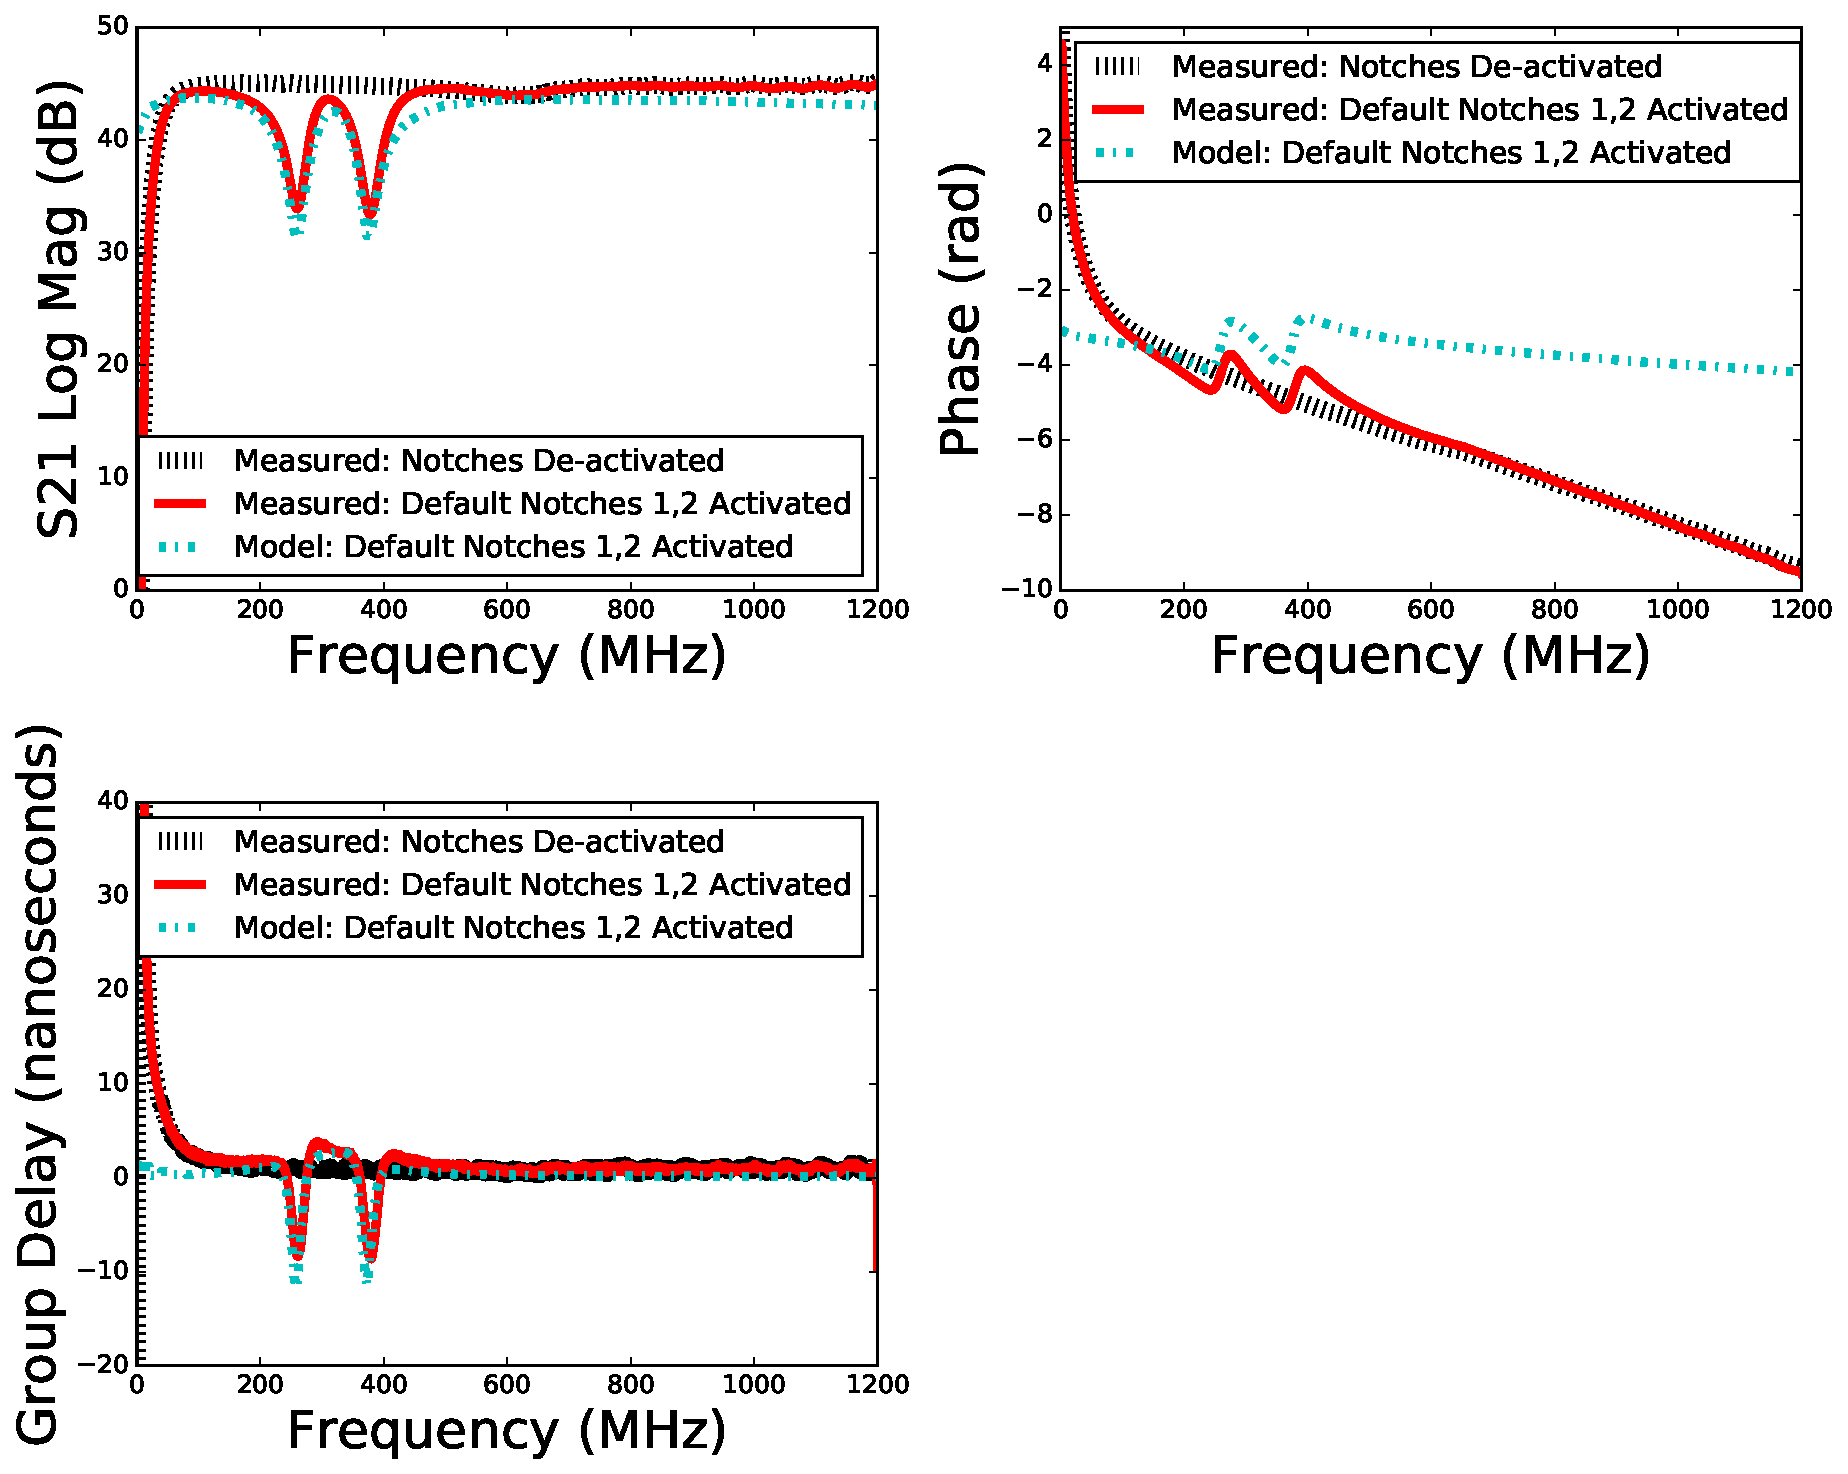
\includegraphics[width=1.0\textwidth]{figures/12measured_model_gain_phase_gd.pdf}
\caption{The gain, phase and group delay as measured and simulated for a TUFF channel with the first two notch filters activated (most common configuration used during the ANITA-4 flight) and all notch filters de-activated.}
\label{tuff_measured_model}
\end{figure}

\subsection{Microcontroller}

We use an ultra-low-power microcontroller, specifically a MSP430G2102 by Texas Instruments.
This features a powerful 16-bit Reduced Instruction Set Computing (RISC) central processing unit (CPU). 
There are five low-power modes optimized for extended battery life. 
The active mode consumes $220\,\mu\mbox{A}$ at $1\,\mbox{MHz}$ and $2.2\,\mathrm{V}$. 
The standby mode consumes only $0.5\,\mu\mbox{A}$ and the RAM retention-off mode consumes $0.1\,\mu\mbox{A}$.
The digitally-controlled oscillator allows wake-up from low-power modes to active mode in less than 
$1\,\mu\mbox{s}$. 

During the ANITA-4 flight, commands could be sent using the SIP connection to set the 
state of the variable capacitor of each \gls{tuff} notch filter via the microcontroller 
of that channel. 
This was done in real time if a re-tune of a notch filter was necessary to mitigate CW interference.
Commands could be sent to de-activate or activate a notch filter using the switch associated with each notch. 
Each microcontroller has the capability to communicate over universal serial communication interface.


\section{Impact of the TUFF boards}

The \gls{tuff} boards had a large impact on the livetime of \gls{anita}. 
There are two types of livetime in ANITA, which are described below.

\paragraph{Digitization livetime} 

In \gls{anita}, deadtime due to digitization by all four \gls{lab} chips of the SURF board is recorded by 
the TURF board, as illustrated in Figure~\ref{system}. 
This deadtime is recorded as a fraction of a second. Digitization livetime per second can be 
obtained by subtracting this from one. 
Increasing the digitization livetime increases the probability of receiving \gls{rf} signal due to an \gls{uhe} neutrino. 

\paragraph{Instrument livetime} 

At any given time, the digitization livetime multiplied by the fraction of unmasked phi sectors (after accounting for channel-masking) gives us the instrument livetime per second. 
In other words, instrument livetime accounts for the fraction of observable ice in azimuth after accounting for masking. 

\subsection{3x instrument livetime}

The most significant impact of the \gls{tuff} boards was the great reduction in the need for masking to mitigate noise during the \gls{anita}-4 flight as compared to \gls{anita}-3. This can be seen in Figure~\ref{masking}. The striking reduction in masking and increase in digitization livetime, as a result of implementing the \gls{tuff} notch filters, contributed to over 91.3\% instrument livetime in \gls{anita}-4 compared to the 31.6\% in \gls{anita}-3.
The performance and impact of the \gls{tuff} boards are described in detail in ~\cite{tuff}, along with visuals comparing the digitization and instrument livetime, thresholds and masking in \gls{anita}-3 and \gls{anita}-4. 

\begin{figure}
\centering
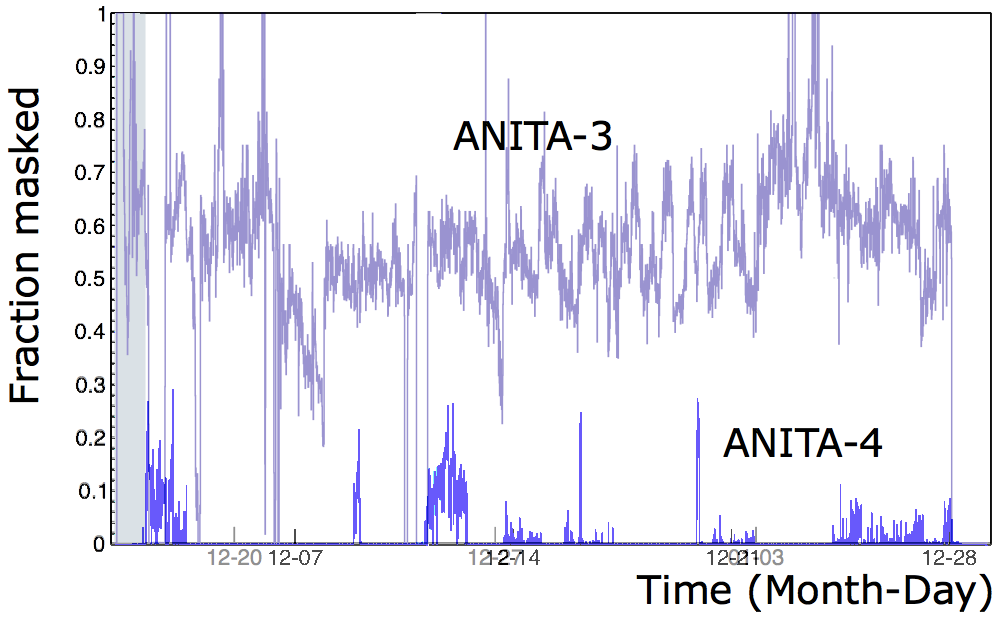
\includegraphics[width=1.0\textwidth]{figures/masking_compare.png}
\caption{Fractional masking implemented in the ANITA-4 and ANITA-3 (faded) flights as a function of time. The TUFF notch filters helped to reduce the need for masking and thereby, tripled the instrument livetime of the experiment.}
\label{masking}
\end{figure}

\begin{figure}
\centering
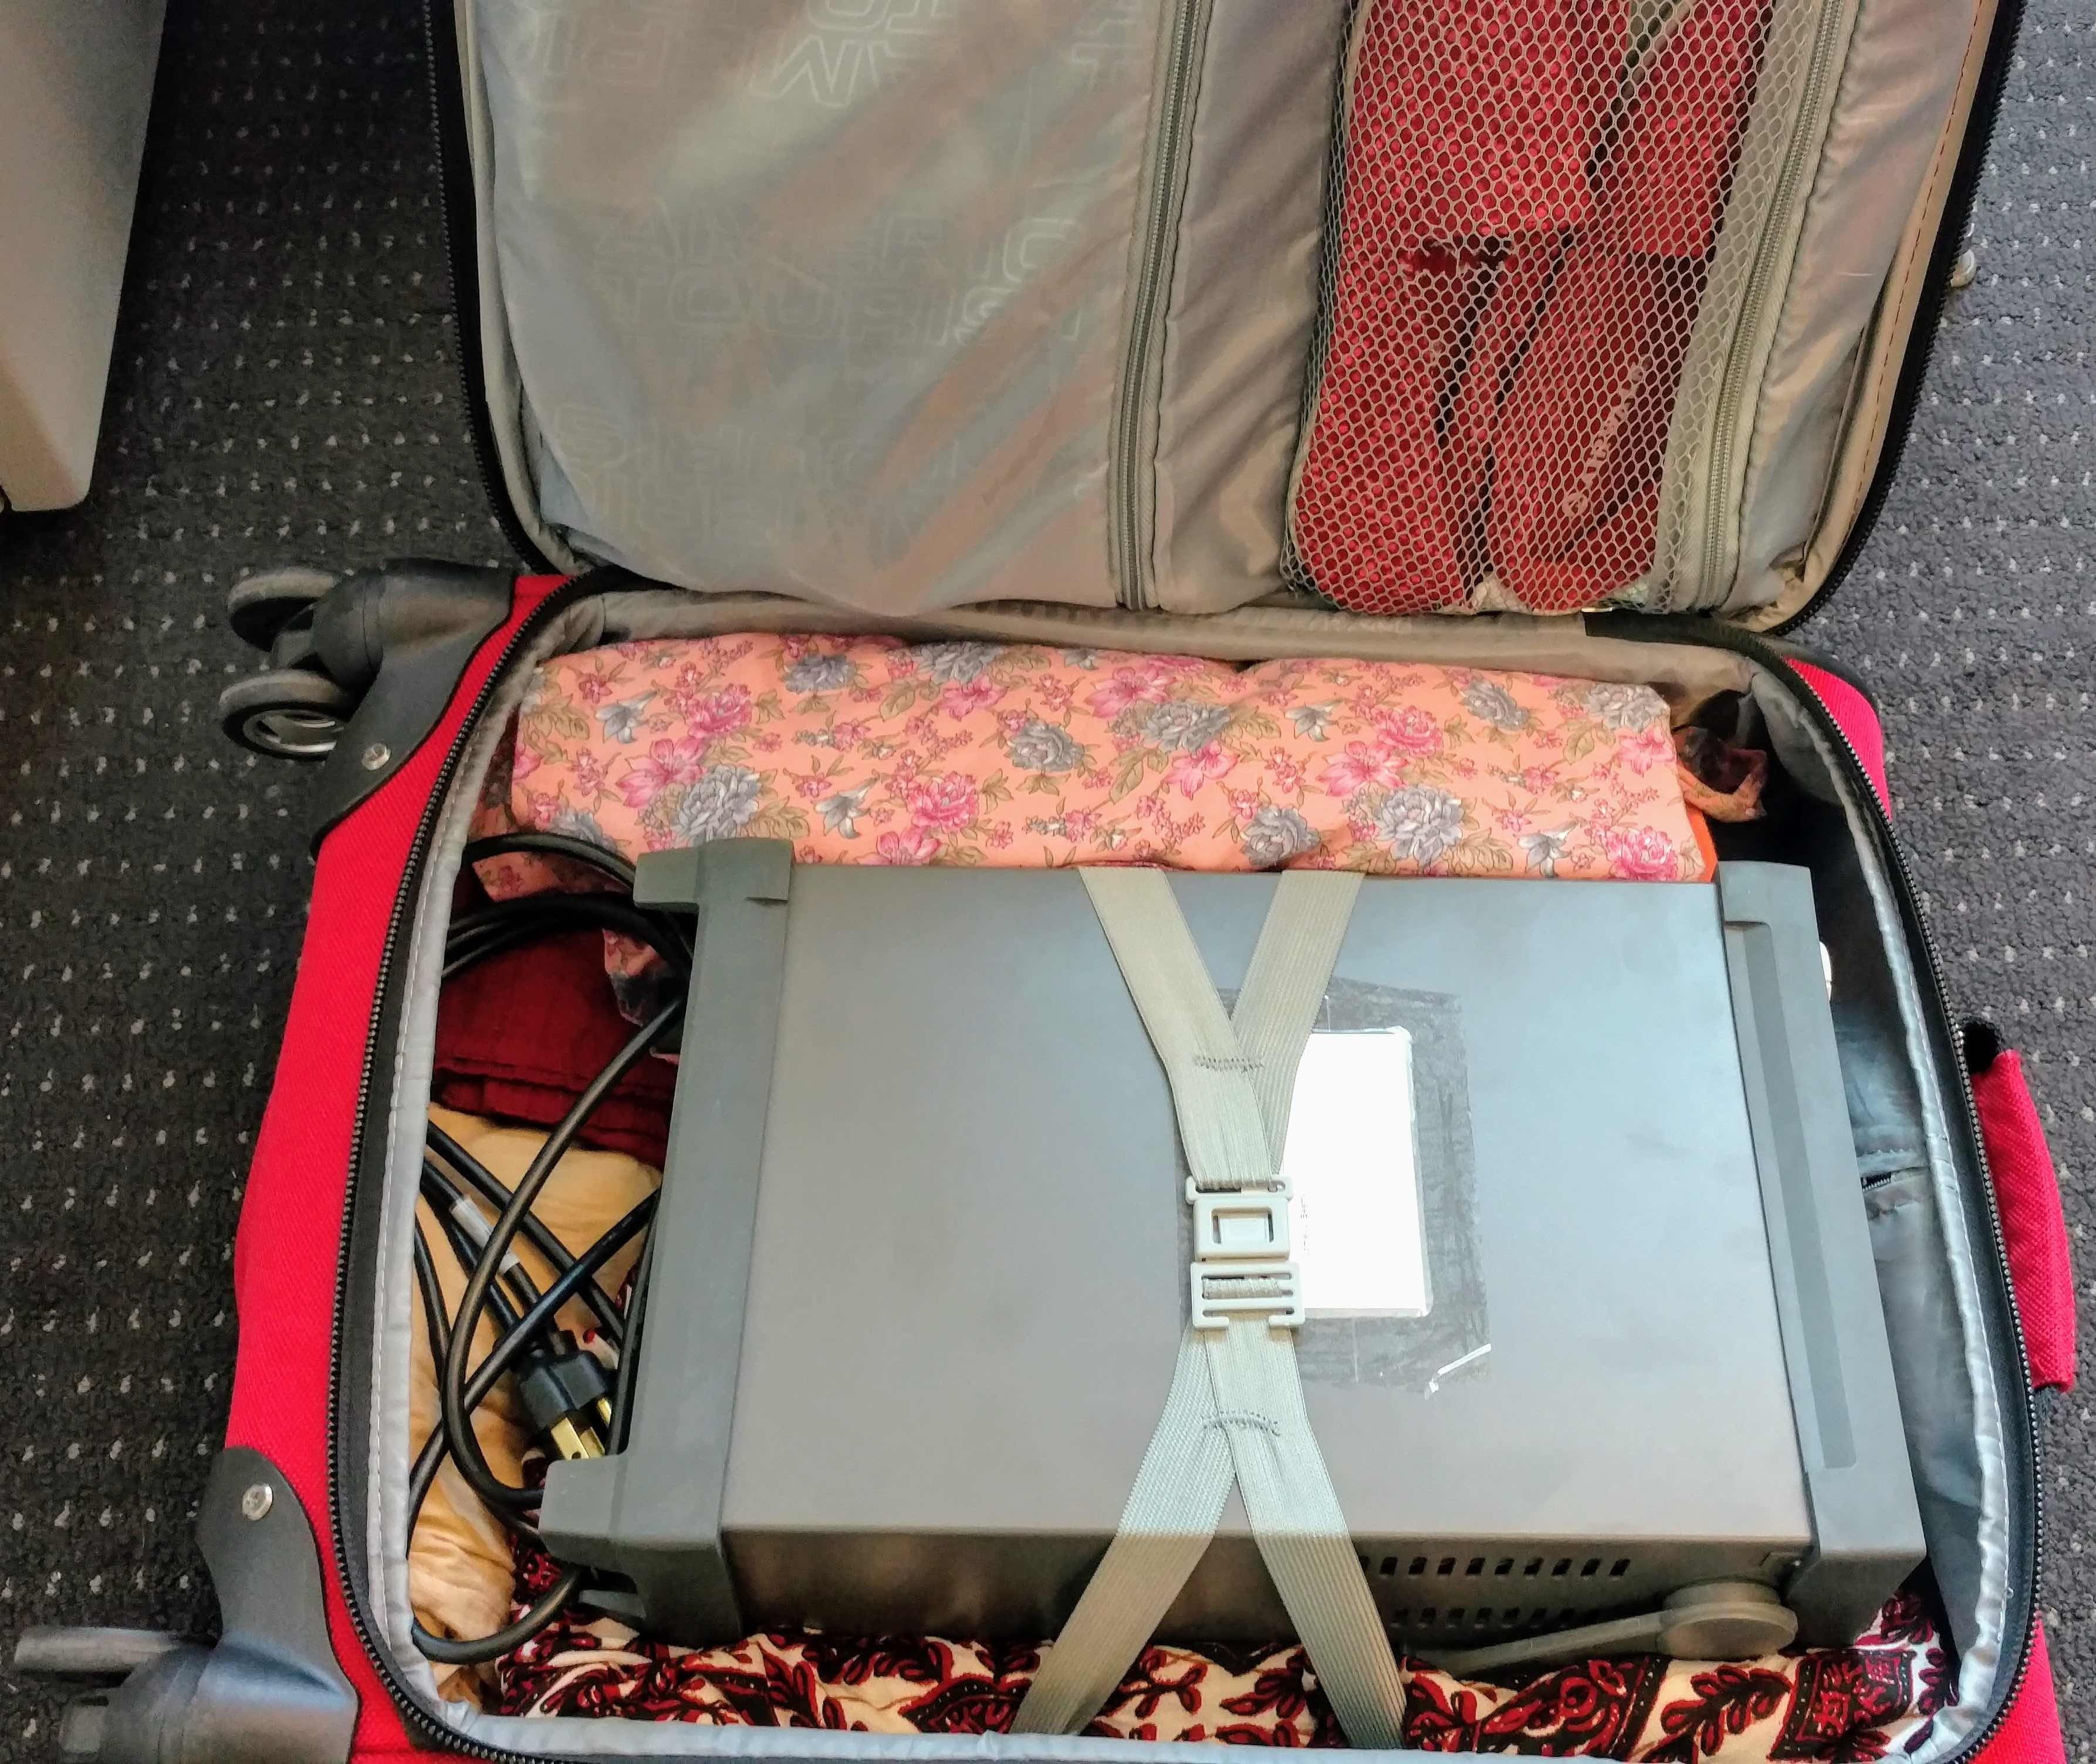
\includegraphics[width=1.0\textwidth]{figures/bag_for_palestine.jpg}
\caption{Bonus: This is the bag I packed for my trip to Palestine, TX, for the hang test of ANITA-4. I packed my own power supply. TUFF boards needed to be tested in Palestine for the integration and hang test, and they needed power. I thought it pertinent to carry my own as other folks' power supplies simply cannot be trusted, especially in challenging situations. This is from Jim Beatty's stash of lab equipment that he may let you borrow for such occasions. The highlight is I got this through airport security by telling the officers all about ANITA!}
\label{palestine_bag}
\end{figure}